\documentclass[11pt]{report}
\usepackage[a4paper,margin=2.5cm]{geometry}
\usepackage[T1]{fontenc}
\usepackage{lmodern}
\usepackage{microtype}
\usepackage{underscore}
\usepackage{booktabs}
\usepackage{array}
\usepackage{longtable}
\usepackage{enumitem}
\usepackage{amsmath,amssymb}
\usepackage{xcolor}
\usepackage{listings}
\usepackage{tikz}
\usetikzlibrary{arrows.meta,positioning,calc,shapes.multipart,fit,backgrounds}
\usepackage{caption}
\usepackage[hidelinks]{hyperref}

\definecolor{grsblue}{HTML}{1F4E79}
\definecolor{grsbg}{HTML}{EEF3F8}
\newcommand{\code}[1]{\texttt{\small #1}}
\lstset{basicstyle=\ttfamily\footnotesize,breaklines=true,columns=fullflexible,frame=single,framesep=4pt,backgroundcolor=\color{grsbg}}
\setlength{\parskip}{0.4em}
% Let long file paths / identifiers set without overrunning the margin.
\sloppy
\emergencystretch=3em

\title{\textbf{Architecture of the Grassroots Networking Transport}}
\author{}
\date{}

\begin{document}
\maketitle
{\small\noindent\emph{This chapter documents \texttt{main} at commit \texttt{7e936ba}. Every factual claim is grounded in the source. File references name the file and the symbol; line numbers are deliberately omitted, because they drift with every commit and a stale line number is worse than none.}}
\tableofcontents
\chapter{Architecture of the Grassroots Networking Transport}


\section{Introduction, Scope \& Design Philosophy}

Grassroots Networking is a \emph{peer-to-peer messaging transport}: a thin layer whose sole responsibility is to move opaque payloads between devices, addressed by cryptographic identity, over two very different media. It is deliberately \emph{not} an application. There is no notion of a chat room, a contact list, a conversation, or a user interface anywhere in its contract; those concepts belong to the applications that sit on top of it. The system's own \code{pubspec.yaml} describes the package (\code{grassroots_networking}, version \code{0.1.0}) as a transport for GSG, the Grassroots Social-Graph application, and the formal specification frames the whole effort as a networking API meant to replace the madGLP \code{IsolateManager} so that GLP agents can run on separate physical devices and communicate directly, peer-to-peer, over a medium-agnostic substrate (\code{docs/GLP_Networking_API/sections/introduction.tex}, \code{docs/GLP_Networking_API/sections/api.tex}). Everything in this chapter should be read through that lens: the layer is plumbing, and its correctness is judged by whether packets reach the right identity, sealed, over whichever medium is available.

\subsection{Design Philosophy}

Four principles, drawn from the project's engineering charter and the GLP specification, shape every decision that follows.

\begin{itemize}
  \item \textbf{Opportunistic mesh delivery.} Over Bluetooth Low Energy (BLE) the transport is a multi-hop \emph{opportunistic mesh}: a node that receives a packet not addressed to it decrements the TTL once (dropping it at zero) and takes the packet \emph{into custody}, and nodes \emph{store-carry-forward} — caching every such transit packet and conveying it onward only when a neighbour asks for it by packet ID in a sealed sync exchange. Nothing is ever pushed: a held packet reaches a recipient (or another carrier) through that request-driven exchange, not through a rebroadcast. This lets a user reach a friend who is not a direct neighbor. The Internet transport, by contrast, stays \emph{direct} point-to-point. Crucially, relaying is not friend-gated and not authenticated hop-by-hop: a relay carries sealed bytes it cannot read, addressed only by recipient identity.
  \item \textbf{Identity is a key pair.} Every device holds an Ed25519 key pair, and the 32-byte public key \emph{is} the peer's globally unique identity, used for addressing, authentication, and signing, persistent across sessions (\code{docs/GLP_Networking_API/sections/api.tex}). Nicknames are cosmetic; all trust flows from cryptographic verification. This is why \code{send} rejects any recipient key that is not exactly 32 bytes (\code{lib/src/grassroots_network.dart}).
  \item \textbf{Two transports, one interface.} BLE covers nearby peers with no Internet; the Internet transport (UDP via UDX, with NAT hole-punching) covers the globe. Both surface the same abstraction to the coordinator — connect, send, receive, disconnect — and BLE is preferred when both are usable (\code{lib/src/grassroots_network.dart}). The two transports are strictly independent: losing or disabling one has zero effect on the other's reachability state.
  \item \textbf{Clean breaks, not compatibility shims.} Because there are no deployed installations in the wild, the project renames, restructures, and breaks wire formats whenever doing so improves the design, rather than carrying legacy decoders or dead code. This principle is not rhetorical — the wire format was recently and deliberately broken (see below), and decoders are written to \emph{reject} malformed or truncated payloads rather than tolerate a hypothetical older version.
\end{itemize}

\subsection{A Corrected Layered Model}

The system is organized as a stack. An application such as GSG never touches radios directly; it calls the \code{GrassrootsNetwork} coordinator, which owns the public API and mediates every layer beneath it.

\begin{verbatim}
+-------------------------------------------------------------+
|  GSG application (chat, social graph, GLP agents)           |
|    consumes: send / onMessageReceived / onPeerConnected     |
+-------------------------------------------------------------+
|  GrassrootsNetwork coordinator  (public API + orchestration)|
|    send(pubkey, payload) . broadcast . onReceive . getPeers |
+---------------------------+---------------------------------+
|  Mesh Router              |  Noise Session Layer            |
|   request-driven relay,   |   Noise_XX_25519_ChaChaPoly_    |
|   seen-set dedup,         |   SHA256; sessions keyed by     |
|   DTN store-carry-forward |   peer pubkey; trial-decrypt    |
+---------------------------+---------------------------------+
|  Transport abstraction  (sendToPeer/broadcast, dataStream)  |
+---------------------------+---------------------------------+
|  BLE mesh transport       |  Internet (UDP/UDX) transport   |
|   dual-role GATT,         |   direct point-to-point,        |
|   neighbor-local ANNOUNCE |   NAT hole-punch via friends    |
+---------------------------+---------------------------------+
|  OS radios: Bluetooth LE stack       /      UDP sockets     |
+-------------------------------------------------------------+
\end{verbatim}

The coordinator (\code{lib/src/grassroots_network.dart}) wires together a \code{ProtocolHandler}, a \code{FragmentHandler}, a \code{NoiseSessionManager}, a \code{MessageRouter}, and a \code{SignalingService}, and exposes the specified surface: \code{initialize}/\code{start}/\code{stop}, \code{send}, \code{broadcast}, \code{getPeers}, \code{isPeerReachable}, and the callbacks \code{onPeerDiscovered}, \code{onPeerConnected}, \code{onMessageReceived} (\code{lib/src/grassroots_network.dart}). Two facts about the layering are load-bearing throughout the chapter. First, the mesh router and the Noise session layer are peers, not one atop the other: the router dispatches packets by their \emph{outer} type and, for a sealed packet addressed to us, asks the session layer to \code{trialDecrypt} it against its sessions, most-recently-used first, until one opens it — the AEAD tag, not any header field, identifies the sender (\code{lib/src/grassroots_network.dart}). Second, sessions are keyed by peer public key, not by transport path, so a Noise session survives a change of relay path or even the loss of a whole transport; \code{stop} tears down transports but deliberately keeps sessions (\code{lib/src/grassroots_network.dart}).

\subsection{System Context}

An outbound message is sealed to the recipient's Noise session and, on BLE, written directly to the recipient when it is a connected neighbor and otherwise held for later; either way the send succeeds as soon as those sealed packets are in the sender's own DTN memory buffer — whether a copy went on the air right now decides only whether the message is shown as \emph{sent} or stays \emph{queued}, because packets nobody was in range to hear are still held for the next sync exchange. If no session exists the send \emph{fails immediately} --- no packet is created, no plaintext is held anywhere, and the user retries once the peer is actually reachable; a message may only ever be created toward a recipient we hold a Noise session with. There is no separate retry queue and no ACK-timeout re-send: redelivery happens exclusively through the sync exchange each time a pairing forms (see \emph{Mesh Routing}). Inbound, a peer is only reported \emph{connected} once an authenticated Noise session exists — reachability is gated on cryptographic authentication, not on a mere radio contact (\code{lib/src/grassroots_network.dart}). Presence and identity ride on a separate, non-relayed channel: the self-signed ANNOUNCE, a neighbor-local broadcast (TTL 1) whose payload carries the full public key, nickname, and an Ed25519 signature over that body (\code{lib/src/grassroots_network.dart}). ANNOUNCE is the \emph{only} packet signed in the clear on the wire; all message, ack, read-receipt, and signaling traffic authenticates end-to-end by decrypting under a verified Noise session, never by a per-packet signature. (One signed object does travel sealed inside that traffic — the inviter-signed invite blob an invitee presents in an \code{INTRODUCE} — but it is a capability that authorizes first contact, not a packet authenticator; see \emph{Facilitators}.)

\subsection{Roadmap}

The remainder of this chapter builds outward from these foundations. \emph{Identity, Trust \& the Security Model} develops the key-pair identity, the sender-anonymous envelope, and why relaying is unauthenticated by construction. \emph{Wire Format, Packets \& the Data Model} specifies the 54-byte header and the sealed \code{SecureFrame} that now carries content type and fragmentation inside the ciphertext. \emph{Transport Abstraction \& the BLE Mesh Transport} covers the common interface and the mandatory dual-role BLE design, and \emph{The Internet Transport \& NAT Traversal} covers the UDX path, address candidates, and hole-punching. \emph{Mesh Routing} details request-driven conveyance, the seen-packetId set (\code{SeenPackets}) that deduplicates it, the DTN memory buffer that makes store-carry-forward work, and its sealed GCS sync exchange. \emph{The Noise Session Layer} covers the \code{Noise_XX} handshake, trial-decrypt, and the AAD construction. \emph{State Management} explains the Redux projection, and \emph{Instrumentation} describes the tracing and testbed machinery that produces the measured numbers this chapter relies on. Later sections walk through end-to-end interactions and close with design decisions, trade-offs, and future work.

\subsection{Lineage and a Warning about Stale Documentation}

The transport descends from the Bitchat protocol. That lineage is now fully retired in the repository --- the README describes the current system, a set of Bitchat-era agent instructions that still forbade relaying and store-and-forward outright has been deleted, and the last dead artefact, \code{lib/src/proto/bitchat.proto}, has been removed along with it --- but it is worth recording, because it explains why so much of this design reads as a deliberate reversal: the ancestor delivered only to peers in direct range and never forwarded on anyone's behalf.

Two scoping notes anticipate common misreadings. First, \emph{rendezvous servers no longer exist}: the \code{bootstrap\_anchor} package, \code{RendezvousServerSettings} and the \code{RV\_LIST} plumbing were deleted outright, and their role is now played by well-connected friends plus signed \code{grassroots://} invite links, both shipped (see \emph{Facilitators}). Second, the multi-hop Noise handshake between peers who have never been in direct range remains future work --- handshakes are neighbor-local (TTL~1). Where this chapter describes a mechanism it describes what the code does; where it labels something future work, that work is not shipped. This edition was regenerated against the source rather than edited from memory: the previous one drifted an entire subsystem out of date before anyone noticed.


\begin{figure}[htbp]\centering
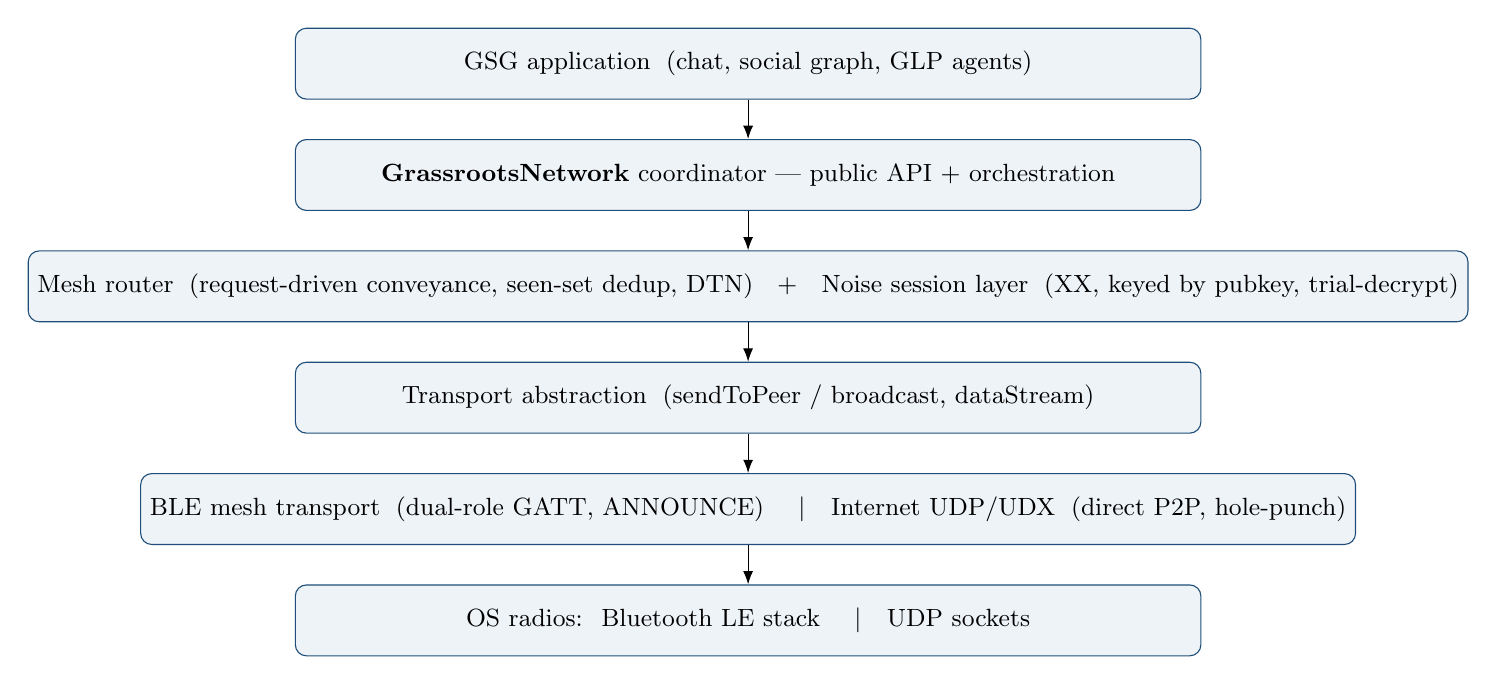
\begin{tikzpicture}[font=\small,node distance=5mm,
  layer/.style={draw=grsblue,fill=grsbg,rounded corners,minimum width=11.5cm,minimum height=9mm,align=center}]
  \node[layer] (app) {GSG application \;(chat, social graph, GLP agents)};
  \node[layer,below=of app] (coord) {\textbf{GrassrootsNetwork} coordinator --- public API + orchestration};
  \node[layer,below=of coord] (mid) {Mesh router \;(request-driven conveyance, seen-set dedup, DTN) \; + \; Noise session layer \;(XX, keyed by pubkey, trial-decrypt)};
  \node[layer,below=of mid] (abs) {Transport abstraction \;(sendToPeer / broadcast, dataStream)};
  \node[layer,below=of abs] (tx) {BLE mesh transport \;(dual-role GATT, ANNOUNCE) \quad$|$\quad Internet UDP/UDX \;(direct P2P, hole-punch)};
  \node[layer,below=of tx] (os) {OS radios: \;Bluetooth LE stack \quad$|$\quad UDP sockets};
  \foreach \a/\b in {app/coord,coord/mid,mid/abs,abs/tx,tx/os} \draw[-{Latex}] (\a) -- (\b);
\end{tikzpicture}
\caption{The layered architecture. The coordinator owns the public API; the mesh router and Noise session layer sit beneath it as peers; two transports share one abstraction.}
\label{fig:layers}
\end{figure}


\section{Identity, Trust \& the Security Model}

The security model of the Grassroots transport is built on a single, deliberately austere primitive: a device's cryptographic key pair \emph{is} its identity. Everything else — trust decisions, session authentication, sender anonymity, and the two distinct trust boundaries described below — is derived from that key pair rather than from any server-issued credential, account, or transport-level address. This section explains what that identity is, how it authenticates a Noise session, how the sender-anonymous mesh envelope constrains what an adversary can learn, and how first contact is gated. It closes with the threat model and the clearly-labelled future redesign of the handshake.

\subsection{Cryptographic identity}

Every device holds an Ed25519 key pair, generated once on first launch (\code{GrassrootsIdentity.generate}) and persisted by the application layer. The 32-byte Ed25519 public key is the peer's canonical identity; the 64-byte private key (32-byte seed concatenated with the public key, per \code{lib/src/models/identity.dart}) never leaves the device. It serves two purposes: signing ANNOUNCE bodies, and deriving the peer's Noise X25519 static key via the birational map (libsodium's \code{skToCurve25519}, \code{noise\_session\_manager.dart}) --- the derivation on which every Noise session in the next subsection rests. Nicknames are purely cosmetic — a mutable display string carried in ANNOUNCE — and carry no authority; two peers with the same nickname are still distinct identities, and a mismatched nickname never overrides the key-based identity.

The public key also seeds BLE discovery. Each device advertises a service UUID whose \emph{fixed} 8-byte Grassroots prefix (the first 8 bytes of \code{SHA-256("grassroots")}) marks it as a Grassroots device, followed by an 8-byte suffix that rotates every 15 minutes (\code{deriveServiceUuidForSlot}: the first 8 bytes of \code{SHA-256("grassroots ble suffix" | pubkey | slot)}, where \code{slot} is wall-clock time divided by a 15-minute \code{bleSlotDuration}). The rotating suffix is an \emph{unlinkable} recognition hint — a peer who knows the key recomputes the current and adjacent slots' UUIDs to recognise the device and pre-filter scans, while a third party who does not know the key sees a beacon that changes every slot and cannot track it — but it is explicitly \emph{not} an authorization proof: it is only a truncated hash, and the full public key is authenticated separately by the signed ANNOUNCE.

\emph{Experiment note.} The rotation is gated behind \code{GrassrootsIdentity.bleSlotRotationEnabled}, which is currently \code{false} for the field-experiment campaign: rotation's destructive re-advertise drops live links every slot, which perturbs exactly the link-establishment and mesh-scale quantities the testbed measures. With the flag off, \code{currentBleSlot()} pins to \code{0} and each device presents one stable UUID. This is a measurement accommodation, not a design change --- the rotating beacon is the architecture, and setting the flag back to \code{true} restores it.

\subsection{Noise sessions and the birational static-key check}

End-to-end confidentiality and authentication run over Noise, pattern \code{Noise\_XX\_25519\_ChaChaPoly\_SHA256} (\code{lib/src/session/noise_session_manager.dart}). A crucial design decision links the two key systems: the Noise \emph{static} key is not an independent secret but the X25519 form of the Ed25519 identity, derived via the standard birational map (libsodium's \code{crypto\_sign\_ed25519\_sk\_to\_curve25519} / \code{pk\_to\_curve25519}). Because the public half of the static is a deterministic public function of the Ed25519 public key, any peer that knows a counterpart's identity can \emph{recompute} the static it should present.

This is exactly what \code{\_verifyRemoteStatic} does. During the XX handshake the remote's static key is delivered encrypted inside messages 2 and 3; on receiving it, the local side recomputes the expected X25519 static from the peer's claimed Ed25519 identity and compares (in constant time) against what Noise delivered. A peer that presents a static not belonging to the identity it claims — or a tampered transcript — fails the check, and the handshake is aborted and the session entry discarded. Handshake authenticity therefore rests on the Noise transcript \emph{plus} this static binding; it is what ties the ephemeral Noise session to a durable, verifiable Ed25519 identity. Sessions are keyed by the peer's Ed25519 public key, never by transport path, so one session serves both the direct UDP path and any relayed BLE path and survives changing relay routes.

\subsection{The sender-anonymous envelope and its consequences}

The outer packet header is 54 bytes and carries only the \emph{recipient} public key (32 bytes), plus type, TTL, packet ID, and payload length (\code{lib/src/models/packet.dart}). There is no sender field and no whole-packet signature. This single structural choice cascades through the whole security model:

\begin{itemize}
  \item \textbf{ANNOUNCE is the only signed \emph{packet}.} The wire \code{PacketType} enum has exactly three values — \code{announce}, \code{noiseHandshake}, and \code{secure}. ANNOUNCE is the one packet whose sender is \emph{meant} to be visible: it is a neighbour-local, non-relayed presence broadcast whose payload ends with an Ed25519 signature over the body (pubkey, a flags byte, nickname, address candidates), verified hop-locally in \code{decodeAnnounce} against the embedded pubkey. Every other packet carries no wire signature at all. One qualification, because the phrase ``the only signature'' recurs in this chapter: a signed \emph{invite blob} is also Ed25519-verified on receipt (\code{Invite.decode} in \code{lib/src/signaling/invite.dart} throws \code{Invite signature invalid}), but that signature authenticates a \emph{capability carried inside} a sealed payload, not a packet — see \emph{Facilitators}.
  \item \textbf{Authentication is end-to-end, inside Noise.} A \code{secure} packet is an opaque, session-sealed envelope. Its logical content type and any fragmentation live \emph{inside} the encrypted payload as a \code{SecureFrame} (\code{[contentType][fragIndex][fragCount][messageId][chunk]}), so a relay never learns the message class — it sees only a \code{secure} blob addressed by recipient. The recipient trusts the content solely because it decrypts under a Noise session whose static was verified above; the ChaCha20-Poly1305 AEAD tag is the authentication.
  \item \textbf{Trial-decrypt demultiplexing.} Because the envelope names no sender, the recipient cannot look up the right session by header. Instead \code{trialDecrypt} attempts decryption against every active session in turn; the AEAD tag identifies the correct one (a wrong session simply fails the tag and is skipped), and the matching session's peer key is returned as the recovered sender.
  \item \textbf{AAD excludes mutable fields.} The application AAD (\code{\_applicationAad}) binds the constant \code{secure} type byte, the sender pubkey, the recipient pubkey, and the 16-byte packet ID — but deliberately \emph{excludes} TTL, which every relay mutates and which therefore cannot be authenticated end-to-end. TTL is now the whole of that exclusion: the header's former 4-byte timestamp has been removed outright, so the envelope contains exactly one relay-mutable field. The content type is nonetheless authenticated, because it sits inside the AEAD-protected plaintext.
  \item \textbf{Bounded replay window.} Each transport session tracks received 64-bit nonces and rejects a repeat as a replay, retaining the most recent 2048 nonces (\code{\_rememberReceivedNonce}) — a bounded window that resists replay without unbounded memory growth.
\end{itemize}

\subsection{Cold-call trust and two trust boundaries}

First contact from a stranger is governed by a \code{ColdCallTrustLevel} setting (\code{lib/src/store/settings\_state.dart}). In \code{open} mode a device completes the BLE ANNOUNCE exchange with unknown nearby peers, permitting cold-call first contact; in \code{closed} mode it does not complete ANNOUNCE with unknown peers, and friend-only metadata is withheld until a verified ANNOUNCE has authenticated an accepted friend. \textbf{The shipped default is \code{open}} --- the \code{SettingsState} constructor default, and therefore \code{SettingsState.initial}, is \code{ColdCallTrustLevel.open}. (A stored settings blob that fails to name a level decodes to \code{closed}; that fallback governs only deserialisation of an unrecognised value, not a fresh install.) The permissive default is what makes the mesh usable out of the box, and it is worth stating plainly rather than assuming the conservative option.

Two distinct trust boundaries coexist, and it is important not to conflate them:

\begin{itemize}
  \item \textbf{Open BLE relay.} The mesh relays \code{secure} packets for \emph{arbitrary} recipients — a relay forwards sealed, recipient-addressed bytes for peers it has no relationship with. It can do so safely precisely because it learns neither the sender nor the content; relaying is unverified by construction, bounded instead by TTL, dedup, and rate limits (discussed in the mesh routing section).
  \item \textbf{Friend-only UDP signaling.} Internet hole-punch coordination is, by contrast, friend-gated. A device only registers friends' addresses, only answers address queries for friends, and only dispatches \code{PUNCH\_INITIATE} to friends: \code{signaling\_service.dart} guards these paths with explicit \code{isFriend} checks — a per-call target guard, plus \code{\_isTrustedSignalingSender} on the inbound side, which admits a sender only if the peer store knows it as a friend (or as a transiently trusted invite introducer) (e.g. it refuses to mediate when \code{targetPeer == null || !targetPeer.isFriend}). This boundary exists because signaling exposes addresses — real metadata — whereas the BLE mesh only ever forwards sealed content. The gate has one deliberate hole, described in \emph{Facilitators}: \code{INTRODUCE} is dispatched \emph{before} the friend check, because an invite redemption is precisely the case of a stranger who must be heard. It is safe because it is self-authorizing — the receiver verifies the inviter's signature over the embedded invite — rather than because the sender is trusted.
\end{itemize}

\subsection{Threat model}

Against a relay or passive BLE observer, the design confines the leak to routing metadata. Such an adversary learns the \emph{recipient} of a \code{secure} packet, its size, TTL, and packet ID — plus its own observation time, since the header carries no timestamp of its own — and can therefore perform traffic-flow and dedup analysis. It does \emph{not} learn the sender (absent from the envelope), the message content, or even the message \emph{class} — message, ack, receipt, and signaling are indistinguishable once sealed. It cannot forge or replay content: forgery fails the AEAD tag under a session it does not hold, and replay is caught by the 2048-nonce window. ANNOUNCE, being signed, cannot be spoofed to impersonate an identity. The residual disclosures — recipient visibility and the fact that ANNOUNCE reveals presence and identity to neighbours — are the accepted, deliberate cost of an open, unverified relay; they are the price of a mesh that reaches beyond direct neighbours without hop-by-hop signatures.

\subsection{Future work: KK/IK handshake redesign}

The current handshake is the interactive Noise XX pattern and is \emph{neighbour-local}: handshake packets are not relayed (TTL~1), so two peers must be in direct BLE range (or on a direct UDP path) to establish a session. A from-scratch multi-hop handshake using the pre-shared-static Noise patterns \emph{IK} and \emph{KK} — which would let a session be negotiated across relays to a peer whose identity is already known — is \emph{not} implemented and is planned future work, to be accompanied by a security audit of the redesigned handshake. Until then, session establishment remains a direct, neighbour-local step even though the resulting session is fully path-independent and survives relaying.

\section{Wire Format, Packets \& the Data Model}

At the base of the transport sits a single on-wire container: the \code{GrassrootsPacket}. Every byte that crosses a Bluetooth or Internet link is one such packet --- the sole exception being the DEBUG/TESTBED raw-throughput blob, whose reserved first byte \code{rawPacketType = 0x7F} is deliberately \emph{not} a \code{PacketType}, so the receiver counts its bytes in the wire ledger and drops it before the parser, measuring the GATT pipe with zero protocol on top (\emph{Instrumentation}). The packet's design encodes the transport's central privacy commitment directly into the header. The header is exactly \textbf{54 bytes} (\code{GrassrootsPacket.headerSize = 54}, \code{lib/src/models/packet.dart}). Its defining property is that it is \emph{sender-anonymous}: it carries the recipient and nothing that identifies the originator. (Earlier editions of this chapter contrasted it against a 154-byte, sender-carrying, whole-packet-signed header documented in the repository README. That README has since been rewritten and now describes the current design correctly, so the contrast no longer has a live referent.)

\subsection*{The 54-byte header, field by field}

The header serialises the following fixed layout, with all multi-byte integers big-endian:

\begin{verbatim}
[0]      type        (1 byte)   0x01 announce | 0x02 noiseHandshake | 0x03 secure
[1]      ttl         (1 byte)   decremented per relay hop, dropped at 0
[2-33]   recipient   (32 bytes) recipient public key; all-zero = broadcast
[34-49]  packetId    (16 bytes) UUID, used for dedup / loop suppression
[50-53]  length      (4 bytes)  payload length
[54..]   payload     (variable) Noise-sealed for secure packets
-------
54 bytes total header
\end{verbatim}

Two absences are the whole point. There is \emph{no sender field} and \emph{no whole-packet signature}. A relay can route a packet toward its \code{recipient} without ever learning who sent it, and — because there is no signature over the header — a relay also \emph{cannot} authenticate the packet it forwards. This is deliberate: hop-by-hop authentication is traded away for sender-anonymity, and the resulting open, unverified relay is instead bounded by \code{ttl} (default 7) and by \code{packetId} deduplication (see the mesh-routing discussion elsewhere in this chapter). An all-zero recipient decodes to the broadcast sentinel.

The header once carried a fourth field --- a 4-byte Unix-seconds \code{timestamp} sitting between \code{ttl} and \code{recipient} --- and it has since been deleted, shrinking the header from 58 bytes to 54 and shifting every field after \code{ttl} down by four. It went because it was \textbf{write-only}: \code{serialize} wrote \code{DateTime.now()} and \code{deserialize} read it straight back into a field nothing consumed. No dedup, expiry, freshness or ordering decision read it --- DTN age expiry uses the store's own local \code{storedAt}, relay dedup uses \code{packetId}, and reassembly uses the inner \code{messageId}. Nor was it authenticated: the application AAD is exactly \code{type + sender + recipient + packetId} (\code{\_applicationAad}, \code{lib/src/session/noise\_session\_manager.dart}), so any relay could rewrite the timestamp freely and no endpoint would notice. Four unauthenticated bytes on every packet --- about 7\% of the old header --- serving only a round-trip test is a cost with no buyer, so they are gone; if a wire timestamp is ever wanted for measurement it belongs inside the seal, where it can be trusted. The \code{length} field, now at offset 50 (\code{GrassrootsPacket.payloadLengthOffset = 50}), doubles as the stream framer: a byte-stream transport such as UDX accumulates bytes until \code{headerSize + length} are present before it treats the buffer as one packet (\code{peekPayloadLength}). The shift is also why the packet id's position became a published constant, \code{GrassrootsPacket.packetIdOffset = 34}: code that slices the id out of a raw buffer without parsing it --- the wire ledger's \code{\_packetIdOf} (\code{lib/src/trace/wire\_ledger.dart}) --- now derives the slice from the packet definition instead of hardcoding byte positions that a header change would silently invalidate.

\subsection*{Three wire types, and why the fourth field moved inside}

The wire \code{PacketType} enum has been deliberately tightened to exactly \textbf{three} values: \code{announce} (\code{0x01}), \code{noiseHandshake} (\code{0x02}), and \code{secure} (\code{0x03}). Everything that is not a presence broadcast or a handshake message is a single, opaque \code{secure} envelope. This refactor is shipped and complete: \code{flutter test} is green at \textbf{782/782}, and there is no second implementation left to migrate — the \code{bootstrap\_anchor} package that once mirrored this wire was deleted along with the rendezvous servers (see \emph{Facilitators}), so no interop gap remains.

The motivation is a metadata leak. The previous wire distinguished \code{secureMessage}, \code{secureAck}, \code{secureSignaling}, and several \code{secureFragment*} types directly in the header — so a relay, which can read the header but never the sealed body, could still tell an acknowledgment from a message from a signaling packet, and could see fragment boundaries. Collapsing all of these to one \code{secure} type closes that leak: a relay now sees only \code{0x03} for \emph{all} sealed traffic and can distinguish neither the message class nor the fragment structure. This is the same class of leak the handshake security audit flagged.

The content type and fragmentation information did not disappear; they \emph{moved inside} the sealed payload, into a \code{SecureFrame} (\code{lib/src/models/secure_frame.dart}). The \code{SecureFrame} is the plaintext that gets sealed into a \code{secure} packet, with a 21-byte inner header:

\begin{verbatim}
[0]      contentType (1 byte)   see the eight values below
[1-2]    fragIndex   (2 bytes)  0-based fragment index
[3-4]    fragCount   (2 bytes)  total fragments; 1 = whole message
[5-20]   messageId   (16 bytes) logical message id (binary UUID)
[21..]   chunk       (variable) this fragment's bytes
\end{verbatim}

\code{ContentType} has \textbf{five} values, and it is worth listing all of them because the sealed envelope is the only place they appear (\code{0x06}--\code{0x08} are retired gaps: \code{0x06} was once a separate sync-request type, \code{0x07}/\code{0x08} the testbed's remote-start signal and armed-time neighbour gossip, deleted when field runs moved to the wall-clock-anchored manual launch):

\begin{verbatim}
0x01 message           application payload (a GSG Block; may be fragmented)
0x02 ack               delivery acknowledgment; chunk = UTF-8 messageId
0x03 readReceipt       read receipt; chunk = UTF-8 messageId
0x04 signaling         hole-punch / address signaling; chunk = SignalingCodec payload
0x05 syncFilter        buffer reconciliation: a GCS filter of the packetIds this
                       node has SEEN, over a creation-time window
\end{verbatim}

The last one matters to the architecture, not just to the enum: \code{syncFilter} carries the entire store-carry-forward reconciliation (\emph{Mesh Routing}), which is why the sync exchange is described there as sealed rather than cleartext.

Because \code{contentType} lives inside the AEAD-protected plaintext, it is authenticated end-to-end for free — the recipient learns the true content class only after a successful decrypt, and no one in between can. The \code{nack} type present in the old enum was removed as dead. Fragmentation is now framing metadata (\code{fragIndex}/\code{fragCount}) rather than a family of wire packet types: a non-fragmented message is simply \code{fragCount == 1}.

\subsection*{Encode/decode discipline: throw, never tolerate}

The codecs follow the project's no-compatibility-shim rule strictly. \code{GrassrootsPacket.deserialize} throws a \code{FormatException} if the buffer is shorter than the 54-byte header or if the declared payload is truncated; \code{PacketType.fromValue} and \code{ContentType.fromValue} throw on any unknown tag rather than falling back; a recipient key that is not exactly 32 bytes throws in the constructor; and \code{SecureFrame.decode} throws when the data is shorter than its 21-byte header. There is no "gracefully handle an older, shorter payload" branch anywhere — since no prior wire version exists in the wild, a malformed payload is malformed, and the decoder says so.

\subsection*{ANNOUNCE: the one signed, non-relayed packet}

\code{ANNOUNCE} is the single exception to sender-anonymity, because presence is precisely a statement about identity. It is neighbour-local (TTL 1, not relayed) and carries a payload-level Ed25519 self-signature. Its payload layout (\code{lib/src/protocol/protocol_handler.dart}) is:

\begin{verbatim}
pubkey(32) + flags(1) + nickLen(1) + nick + candidateCount(2)
           + repeated[ candidateLen(2) + candidate ] + signature(64)
\end{verbatim}

The \code{flags} byte is a single byte, not a version field. Bit~0 is \code{willingToFacilitate}: the peer volunteers to introduce strangers redeeming a friend's invite (\emph{Facilitators}). It rides \emph{inside} the signed body precisely so that a peer's advertised willingness cannot be forged by a neighbour rewriting the advertisement.

\code{decodeAnnounce} strips the trailing 64-byte signature, verifies it over the body against the \emph{embedded} public key, and throws \code{ANNOUNCE signature invalid} on failure; it also rejects payloads below the 96-byte (32+64) floor and any truncated candidate field. This is the only signature the transport verifies on a \emph{packet header or payload framing}; message, ack, read-receipt, and signaling content authenticate purely end-to-end, by trial-decryption against Noise sessions (discussed in the section on the Noise session layer). The one other Ed25519 verification in the system checks an invite blob carried \emph{inside} an already-sealed payload (\code{Invite.decode}), which is a capability check rather than a packet check.

\subsection*{Fragmentation and reassembly as SecureFrames}

Large payloads are split by the \code{FragmentHandler} (\code{lib/src/protocol/fragment_handler.dart}), and its budget is derived from the BLE floor MTU rather than chosen. A fragment is sent as \emph{one} GATT write — the plugin does not split or reassemble, so a sealed packet larger than \code{ATT\_MTU - 3} is silently truncated on the wire and the receiver cannot parse it. Sizing therefore starts from the floor MTU the transport requests, \code{\_bleFloorMtu = 247} (244 usable), and subtracts the fixed per-packet overhead of \textbf{100 bytes} --- 54 (packet header) $+$ 25 (Noise version, nonce and tag) $+$ 21 (frame header):

\[ \code{maxFragmentPayload} = 247 - 3 - 100 - 8 = \textbf{136 bytes} \]

the trailing 8 being margin, which puts a full fragment in a 236-byte packet. That margin is \emph{chosen rather than derived}, and it is worth being explicit about what it buys: 247 is the MTU the transport \emph{requests}, not the one a given pair necessarily negotiates, so a chunk cut to exactly 144 would truncate silently against any peer that settles below 247 --- 8 bytes covers down to a 239-byte MTU. Whether such a peer exists on this hardware has not been measured; the payload arm sweeps 132/264/1200\,B, of which the first sits below the budget and the other two fragment, so no run has yet put a 144-byte chunk on the air. The \code{Raw link: ATT ceiling probe} preset exists to settle it, writing raw blobs at $\text{MTU}-3+\delta$ for $\delta \in \{-8,-4,0,+1,+4\}$ and recording the length that actually arrives; reclaiming the margin would be worth roughly 6\,\% more payload per fragment. \code{fragmentThreshold} is defined to \emph{equal} \code{maxFragmentPayload}, so the threshold and the chunk size are the same number, \textbf{136}: a single frame carries no more than a fragment does. A payload above it is chunked into \code{SecureFrame}s sharing one \code{messageId} and carrying ascending \code{fragIndex} out of a common \code{fragCount}; \code{framesFor(...)} produces the list and the sender emits them \code{fragmentDelay = 20\,ms} apart. Crucially, each fragment is an ordinary \code{secure} packet — reassembly happens \emph{after} decryption, keyed by the inner \code{messageId}, so relays never see fragment structure. \code{accept(frame)} buffers fragments and returns the complete payload once every index has arrived (immediately for a single-fragment message), with a stale-reassembly timeout of \textbf{four minutes} --- sized to outlast the slowest transfer the system allows, roughly 8k fragments at 136\,B and 20\,ms apiece for the $\sim$1\,MB attachment cap, plus slack.

\code{GrassrootsPacket.maxPayloadSize = 446} (computed as $500-54$) still exists in \code{packet.dart} as a nominal single-packet ceiling, but nothing references it: the enforced budget is the \code{FragmentHandler} arithmetic above, against a 247-byte floor MTU rather than the 500 bytes that constant assumed. Treat 446 as vestigial. Note also that relay/loop dedup is keyed on the \emph{outer} \code{packetId}, whereas delivery dedup is keyed on the \emph{inner} \code{messageId} — the two identifiers serve different layers.

\subsection*{The application data model: Blocks}

Above the transport, an application payload is a serialised \code{Block} (\code{lib/src/models/block.dart}) — the unit GSG builds its blocklace from. A \code{Block} is a one-byte \code{type} tag followed by its body, and \code{Block.deserialize} reads \code{data[0]} as the type and treats the remainder as the payload. The current \code{BlockType}s are \code{say} (\code{0x01}), \code{friendshipOffer} (\code{0x02}), \code{friendshipAccept} (\code{0x03}), and \code{friendshipRevoke} (\code{0x05}); value \code{0x04} is a reserved gap. A \code{SayBlock} adds a one-byte \code{subtype}, so its wire form is \code{[0x01 type][subtype][body]}. There are \textbf{three} subtypes, and two of them make attachments \emph{first-class content} rather than an application concern layered on top of text:

\begin{itemize}
  \item \code{text} (\code{0x00}) --- raw UTF-8.
  \item \code{picture} (\code{0x01}) --- \code{[viewOnce:1][mimeLen:1][mime][imageBytes]}. The \code{viewOnce} flag drives the ``render blurred, delete on first view'' behaviour; images are compressed for BLE and stored content-addressed by SHA-256 (\code{lib/src/services/media_service.dart}).
  \item \code{file} (\code{0x02}) --- \code{FileSayBlock}, whose body is \code{[nameLen:2][name][mimeLen:1][mime][bytes]}: a named attachment of arbitrary type, distinct from \code{picture} because it carries a filename and gets no image treatment.
\end{itemize}

No \code{Block} subtype carries a signature; packet-level signing lives only in ANNOUNCE, consistent with the model above.

\subsection*{From app payload to sealed bytes}

The end-to-end path is therefore a clean stack of nested framings. An application constructs a \code{Block} and serialises it. That byte string becomes the \code{chunk} of one or more \code{SecureFrame}s (one if it is within the 136-byte threshold, several otherwise), each tagged \code{contentType = message} and carrying a shared \code{messageId}. Each \code{SecureFrame} is encoded and then \emph{sealed} by the Noise session keyed to the recipient, producing the opaque payload of a \code{secure} (\code{0x03}) \code{GrassrootsPacket} addressed only to that recipient. What finally travels the mesh is a 54-byte anonymous header wrapping ciphertext — the message class, the fragment structure, the sender, and the content all hidden inside the seal, visible only to the two endpoints.

\begin{table}[htbp]\centering
\caption{The 54-byte cleartext wire header (sender-anonymous) and the 21-byte inner \code{SecureFrame} that lives inside the sealed payload.}
\label{tab:frame}
\begin{tabular}{@{}rll@{}}
\toprule
\multicolumn{3}{@{}l}{\textbf{Outer wire header --- 54 bytes, cleartext, sender-anonymous}}\\
\midrule
Offset & Bytes & Field \\
\midrule
0  & 1  & packet type: announce / noiseHandshake / secure \\
1  & 1  & TTL (decremented at each relay hop) \\
2  & 32 & recipient public key (zeros = broadcast) \\
34 & 16 & packet id (dedup / loop prevention) \\
50 & 4  & payload length \\
\midrule
\multicolumn{3}{@{}l}{\textbf{Inner SecureFrame --- 21-byte header, sealed inside the payload}}\\
\midrule
0  & 1  & content type: one of five (message, ack, readReceipt, signaling, \\
   &    & \quad syncFilter) \\
1  & 2  & fragment index \\
3  & 2  & fragment count (1 = not fragmented) \\
5  & 16 & message id (logical id: reassembly + ACK correlation) \\
21 & \emph{n} & chunk (content bytes; the whole payload when fragCount = 1) \\
\bottomrule
\end{tabular}
\end{table}


\section{Transport Abstraction \& the BLE Mesh Transport}

Grassroots exposes exactly one abstraction to the layers above it, and hides two very different radios beneath it. A message router does not know whether the bytes it hands down will travel over Bluetooth to a device in the same room or over the Internet to a device on another continent; it only knows the \code{TransportService} interface. This section describes that interface and its lifecycle, then examines the Bluetooth Low Energy (BLE) transport in depth --- discovery, dual-role convergence, and how packets actually move over GATT.

\subsection{The Unified Transport Interface}

Every transport implements the abstract \code{TransportService} class (\code{lib/src/transport/transport_service.dart}). The interface is deliberately small: type and display metadata, a \code{state} getter, two event streams (\code{dataStream} for inbound bytes, \code{connectionStream} for connect/disconnect events), \code{connectedCount}/\code{isActive} getters, the lifecycle verbs \code{initialize()}, \code{start()}, \code{stop()}, and \code{dispose()}, and the two send primitives \code{sendToPeer(peerId, data)} and \code{broadcast(data, \{excludePeerIds\})}. The interface also carries a small pubkey$\leftrightarrow$peerId association (\code{getPeerIdForPubkey}, \code{getPubkeyForPeerId}), because a transport addresses peers by an opaque, transport-local peer id (a GATT path id for BLE, an address for UDP), whereas the layers above reason in terms of the peer's public key --- its true identity. The two implementations resolve that association differently and neither does it through a shared interface hook: the BLE transport walks the Redux peer list matching \code{bleCentralDeviceId}/\code{blePeripheralDeviceId} (so the mapping is a by-product of the store being updated from a verified ANNOUNCE), while for UDP a peer id \emph{is} its pubkey hex, making the lookup a hex decode.

\code{broadcast} is the transport's fan-out primitive: it writes a packet to every currently-connected peer and returns the count sent, taking an optional \code{excludePeerIds} set to skip chosen peers (for instance the neighbour a gossiped packet arrived from). It is how the \emph{originator} airs its own traffic to all neighbours at once --- its own \code{broadcast}-API messages, ANNOUNCE, and testbed control --- and it is deliberately \emph{not} a relay primitive: relaying no longer rebroadcasts anything (see \emph{Mesh Routing}), it takes transit packets into custody and conveys them only on request. When an exclusion is used on BLE it is resolved to the peer's \emph{identity} rather than to the named path: a pathId names only ONE leg, so excluding just one leg would let the reverse leg of the same pair receive a second copy. The routing logic that decides what to do with an inbound packet (TTL, dedup, store-carry-forward) lives one layer up in the router, not in the transport --- the transport only exposes the fan-out mechanism. This split is the same on both transports, which is what lets the router treat them uniformly.

A transport moves through a fixed six-state lifecycle (\code{TransportState}): \code{uninitialized} $\rightarrow$ \code{initializing} $\rightarrow$ \code{ready} $\rightarrow$ \code{active}, plus the two out-of-band states \code{error} and \code{disposed}. \code{initialize()} advances a transport from \code{uninitialized} to \code{ready} (subscribing to plugin streams and initialising the underlying BLE plugin; permission provisioning happens one layer up, in \code{GrassrootsNetwork}, not inside the transport); \code{start()} advances \code{ready} to \code{active} (it begins advertising and scanning). A single derived predicate, \code{isUsable}, is true exactly when the state is \code{ready} or \code{active} --- both are states in which the transport can carry traffic, the difference being whether it is also actively seeking new peers. It hangs off the enum as an extension (\code{TransportStateX}), not off \code{TransportService}, so it is available anywhere a \code{TransportState} is in hand. \code{dispose()} is terminal: a disposed transport is unusable and cannot be revived.

Two properties of this design are load-bearing for the rest of the system. First, the two transports are strictly independent: BLE and UDP are toggled separately and neither's lifecycle state, peer reachability, or online status is allowed to influence the other's. A peer reachable over UDP stays reachable regardless of what BLE is doing, and vice-versa; consolidation into a single ``is this peer reachable at all'' signal happens above the transport, not inside it. Second, the enum \code{TransportType} has exactly two values --- \code{ble} and \code{udp} --- and both are real transports; there is no third. An earlier WebRTC transport was removed outright, leaving behind no enum member, no service file, and no stub, in keeping with the project's no-legacy discipline.

\subsection{BLE Discovery: A Rotating, Pubkey-Derived Service UUID}

A device makes itself discoverable by advertising a BLE service UUID whose fixed prefix marks it as a Grassroots device and whose suffix is derived from its public key. \code{GrassrootsIdentity.deriveServiceUuidForSlot} (\code{lib/src/models/identity.dart}) concatenates a fixed 8-byte \emph{grassroots prefix} --- the first 8 bytes of SHA-256(\code{"grassroots"}), the constant \code{84c403160871e5ad} --- with the first 8 bytes of \code{SHA-256("grassroots ble suffix" | pubkey | slot)}, where \code{slot} is the wall-clock time divided by a 15-minute \code{bleSlotDuration}, encoded 8-byte big-endian. The derivation throws if the pubkey is shorter than 32 bytes; there is no lenient fallback. The prefix never changes, so a scanner recognises a Grassroots advertisement by prefix-matching. \code{serviceUuidMatchesPubkey}, over the set returned by \code{candidateServiceUuids}, is the recognition primitive the transport uses throughout.

The suffix rolls each slot, for unlinkability: a passive observer who does not know the public key sees a beacon that changes every 15 minutes and cannot track the device across slots, while anyone who does know the key recomputes the suffix and recognises it. Because unsynchronised clocks and slot boundaries would otherwise break recognition, matching is against a set --- the previous, current and next slot's UUIDs (\code{candidateServiceUuids}). The peripheral hosts its GATT data service under whatever slot UUID it currently advertises --- advertisement and GATT service carry the \emph{same} rotating identifier, deliberately, since rotation is what severs a connected stranger's continuity of observation. A 30-second timer (\code{\_maybeReAdvertiseForSlot}) re-advertises at each boundary, rebuilding the peripheral GATT service under the new UUID and dropping its live central links across it. That rebuild is destructive by design, and it is the accepted cost of the privacy property; pinning the GATT service to a fixed UUID to avoid it would hand any scanner a permanent handle and is explicitly rejected.

\emph{Experiment note.} \code{bleSlotRotationEnabled} is currently \code{false} for the field-experiment campaign, because the slot-boundary link drops perturb the establishment-time and mesh-scale measurements. While it is off, \code{currentBleSlot()} pins to \code{0}, \code{candidateServiceUuids} yields a single stable UUID per pubkey (so scan filters stay one entry per peer), and the boundary re-advertise never fires. The mechanism is unchanged and one flag away; treat the rotating beacon as the design and this as a temporary measurement setting.

The GATT characteristic UUID (\code{0000ff01-...}) is the same constant across all peers.

The UUID is a discovery hint, never an authorization proof --- it tells a scanner ``a Grassroots device carrying \emph{this} key is nearby,'' but authentication is established separately by the self-signed, neighbour-local ANNOUNCE (covered in \emph{Identity, Trust \& the Security Model}). Scanning uses the shared grassroots prefix as a service-UUID filter with a continuous window (timeout \code{Duration.zero}) and \code{allowDuplicates: true}, so iOS keeps delivering RSSI and liveness updates rather than reporting each device only once. Because a silently-muted scan is a known BLE failure mode, a watchdog fires every 10\,s and restarts a scan that has heard nothing for the \code{scanSilenceRestart} window (default 30\,s). The restart is not always a plain prefix scan, and neither is the steady-state one. Scan targeting is recomputed on every leg attach/detach and on each such restart (\code{\_reverseLegScanTargets}, \code{\_applyScanTargets}): for every pair stuck peripheral-only --- a live inbound leg with no live or in-flight reverse leg --- that peer's \code{candidateServiceUuids} are installed as \emph{hardware} scan filters, because it is precisely the filterless long-running Android scan that goes mute under load (advertising plus several GATT-server connections), and a peer whose advertising MAC is never surfaced can never be dialed back, stranding the pair single-link. A filterless restart would only re-enter the same mute. In steady state the target set is empty and the scan falls back to the plain prefix scan. Advertising is started with the identity's derived service UUID, the fixed characteristic UUID, and \code{bondless: true}.

\subsection{Dual-Role Convergence Over GATT}

A single GATT link is one-directional at the role level --- one side is central, the other peripheral --- so a Grassroots pair must converge to a \emph{dual-role} connection: two legs, each device central on one and peripheral on the other. This is mandatory; a single-link pair is only ever tolerated as a transient state that the transport keeps trying to upgrade. Path ids are role-prefixed accordingly: \code{central:<remoteId>} for outbound legs we dial, \code{peripheral:<remoteId>} for inbound legs we accept; only \code{central:} paths are ever dialed.

Who dials first is decided by advertisement-driven arbitration rather than by leaving a leg unopened, and \textbf{the election is now platform-neutral for every pair}: the device whose advertised service UUID sorts lower (\code{compareTo < 0}) opens the first central leg, mirroring UDP's ``smaller pubkey initiates.'' \code{\_shouldDialNow} applies this tiebreaker regardless of platform. A cold-start ``first-mover fallback'' (default 5\,s) ensures the non-initiator dials anyway if the expected initiator never moves.

Earlier revisions carried a platform marker for this: iOS devices advertised the fixed local name \code{grs-ios} so peers could yield the first dial to the iOS side, routing around the measured constraint that an iOS central cannot open the \emph{second} link toward a non-iOS peer. \textbf{That marker and the mixed-pair reform it keyed off have been removed} --- the wrong-order reform (an Android tearing down its central leg so a foregrounded iPhone could re-open the pair in the right order) was deleted along with it. The constraint itself has not gone away; what has gone is the special case, and the UUID election plus the fallback now carry every pair. A reader tracing iOS interop should treat this as the open question it is, not as a solved asymmetry.

Two defensive mechanisms guard the connection machinery against the noise of BLE radio-address privacy. The OS rotates a device's radio MAC / resolvable private address roughly every 30\,s, which produces a fresh transport-level path id for the \emph{same} logical peer; the transport suppresses these duplicates, dropping an advertisement from a rotated MAC when a live or in-flight path to the same peer already exists --- matched against \code{candidateServiceUuids} (one entry per peer while slot rotation is off, the current plus adjacent slots when it is on). Separately, the number of simultaneous in-flight central dials is capped at \code{\_maxInFlightCentralDials = 7}: each \code{connectGatt} holds an Android controller slot for roughly 5\,s, so too many parallel dials starve real connections. In closed cold-call mode the transport additionally refuses to dial or connect to any peer whose advertised service UUID does not match an accepted friend's candidate UUIDs.

\subsection{Moving Packets, MTU, and the Foreground Service}

Once legs are up, sending is direct GATT writes. \code{sendToPeer} resolves the named path and returns \code{false} when it is absent or not sendable (tracing a \code{bleSend}/\code{noPath} or \code{notReady} drop rather than failing silently, which used to be the quietest send failure in the codebase); otherwise both send primitives write through one choke point, \code{\_writeToPeer}. \code{broadcast} sorts the ready paths by RSSI descending (paths with unknown RSSI --- peripheral-role, where the OS does not expose remote signal strength --- sort last via a $-100$ fallback but still receive) and then passes them through \code{selectBroadcastTargets}, which keeps \textbf{exactly one leg per peer identity}, preferring the peripheral leg. This is where the one-leg-per-peer-per-write rule described in \emph{Mesh Routing} is actually enforced: the fan-out is over peers, not over paths, so a converged dual-leg pair receives one copy rather than two. The leg the write did \emph{not} choose is still the pair's fallback: when the chosen leg \emph{refuses} a write, \code{\_writeToPeer} retries the same bytes on the pair's other leg (\code{otherLegFor}) and emits a \code{retry} trace record --- its own record type, not a \code{drop}, so a recovered packet is not counted as a lost one, and so the run can measure what the second leg is actually worth. This is not the double-send the one-leg rule forbids: the fallback runs only after a throw, and on both platforms a write throws \emph{before} anything is transmitted (Android's \code{sendCentral} while validating the path and \code{sendPeripheral} when \code{notifyCharacteristicChanged} refuses the buffer; iOS on \code{valueTooLarge} or a full pending queue), so the packet cannot end up on the air twice. It matters most for exactly the leg a conveyance prefers --- the peripheral leg has no queue at all, so it is the one that refuses under load. Two guards bound it: the retry is skipped unless the payload fits the other leg's MTU (the two legs negotiate separately, and retrying onto a leg that will truncate the write would put unparseable bytes on the air and report success), and it is skipped entirely for a path whose identity is not yet known, where there is no way to tell the pair's other leg from a stranger's. A path is eligible only when its plugin state is \code{ready} and \code{path.canSend} is true. Inbound bytes are parsed by \code{GrassrootsPacket.deserialize}; a malformed packet is caught and dropped rather than propagated --- but not silently: it is logged and traced as a \code{bleRx}/\code{deserialize} drop carrying the received length, the peer's negotiated MTU, and an \code{atUsableLimit} flag for a length sitting exactly at \code{mtu - 3}, which is the signature of a write the \emph{sender's} stack clamped and truncated rather than a corrupt or foreign packet. On every central connect the transport requests an ATT MTU of 247 bytes --- the largest most Android stacks negotiate --- because a single ANNOUNCE alone is $\sim$200 bytes, far over the default 23-byte ATT MTU (a 20-byte payload); the effective MTU is whatever the peer accepts, reported back via \code{BlePath.mtu}, and it is the floor from which \code{FragmentHandler} derives its 136-byte budget (\emph{Wire Format}).

Because Android aggressively freezes backgrounded processes, the process is pinned alive by a native foreground service, controlled over the \code{grassroots/foreground_service} MethodChannel (\code{start}/\code{stop}) and declared with the \code{connectedDevice} foreground-service type. It is a no-op on every platform except Android and swallows a missing native handler, so the same Dart code runs unchanged on iOS. Note the ownership: \code{TransportForegroundService} is driven by the \emph{coordinator} --- started in \code{GrassrootsNetwork.start()} once both transports are up, stopped in \code{stop()} --- not by the BLE transport itself, which never references it. The service covers the whole process, not one radio.

\subsection{A Fossil Worth Flagging}

One stale comment deserves an explicit warning to any reader who opens the source. The \code{BleTransportService} class doc still reads ``\emph{Direct delivery only. No relaying, no store-and-forward}'' --- a fossil from before the mesh migration that directly contradicts the project's opportunistic-mesh design. It is technically accurate about \emph{this file}: the BLE transport genuinely contains no relay, conveyance, DTN, TTL, or dedup logic; \code{broadcast} and \code{sendToPeer} only push to directly-connected GATT paths. But the comment misleads about the \emph{system}: multi-hop store-carry-forward --- request-driven conveyance of packets held in the DTN buffer --- lives one layer up in the router (see \emph{Mesh Routing}), and it reaches beyond direct neighbours by taking transit packets into custody and conveying them on request, not by driving the transport to rebroadcast. The comment should be read as describing the transport's narrow responsibility, not the mesh's behaviour.

\section{The Internet Transport \& NAT Traversal}

Where the BLE mesh (described in \emph{The BLE Mesh Transport} and \emph{Mesh Routing}) gives a device local, Internet-free reach through multi-hop store-carry-forward, the Internet transport gives it \emph{global} reach --- but only ever as a \emph{direct}, point-to-point path between the two endpoints. There is no store-carry-forward, no relaying, and no caching on this side: a message to an unreachable peer fails immediately rather than being held (\code{lib/src/transport/udp_transport_service.dart}). Everything that makes the Internet path hard is therefore concentrated in one problem: two mobile devices, each behind a NAT, have to \emph{find} each other and punch a hole through their respective NATs before that direct path can exist. This section covers the transport itself, then the NAT-traversal machinery --- hole-punching, signaling, and the facilitators that broker the punch.

\subsection{The UDX Transport: Sessions, Sockets, and Reframing}

The Internet transport is built on UDX, a reliable stream protocol layered over UDP. Its \code{TransportState} lifecycle follows the two-phase pattern shared with the BLE transport: \code{initialize()} binds the underlying sockets and moves the transport \code{uninitialized}$\rightarrow$\code{initializing}$\rightarrow$\code{ready}, then \code{startMultiplexer()} constructs the \code{UDXMultiplexer} and moves it \code{ready}$\rightarrow$\code{active} (\code{udp_transport_service.dart}). The split matters for hole-punching: raw punch bursts and the multiplexer contend for the same socket, so the transport can hold in \code{ready} (socket bound, multiplexer not yet running) precisely when it wants to read raw punch datagrams itself.

Initialization binds a \code{RawDatagramSocket} for \emph{both} address families --- IPv6 first, then IPv4 --- each on the wildcard address with ephemeral port~0, and each family gets its own socket and its own multiplexer stored in per-family maps. Binding fails only if \emph{neither} family binds. When a single ``active'' socket must be chosen (e.g. for hole-punch sends), IPv6 is preferred, falling back to the first bound family (\code{udp_transport_service.dart}).

An outgoing connection (\code{connectToPeer}) creates a \code{UDPSocket} on the multiplexer, opens a \code{UDXStream} with a transport-wide monotonically increasing stream id, and awaits \code{handshakeComplete} under a default 10-second timeout (\code{\_defaultHandshakeTimeout}). The stream id is \emph{never reused} --- it increments on every connect --- because UDX will refuse a SYN carrying a recently-closed stream id. Failures are classified into \code{UdpConnectFailureKind.\{networkUnreachable, handshakeTimeout, other\}}: a \code{TimeoutException} becomes \code{handshakeTimeout}, and \code{SocketException} codes 101/113/65 (or unreachable-route text) become \code{networkUnreachable}, so the coordinator can distinguish ``no route'' from ``peer silent'' (\code{udp_transport_service.dart}).

Because the wire envelope is \emph{sender-anonymous} (recipient-only, no sender field --- see \emph{The Wire Format}), an incoming stream cannot be attributed from its bytes. The transport therefore keys the fresh connection by a temporary key of the form \code{remoteAddress:remotePort:streamId}, and only once the coordinator verifies the first packet does it call \code{mapIncomingConnectionToPubkey} to bind that temp key to the peer's public key. Established connections are then keyed by pubkey hex --- and since a peer id \emph{is} its pubkey hex, \code{getPubkeyForPeerId} is just a hex decode (\code{udp_transport_service.dart}).

UDX delivers a reliable \emph{byte stream}, not discrete datagrams, so the receiver must recover packet boundaries. A \code{\_PacketFramer} buffers incoming bytes and reframes them into 54-byte-header \code{GrassrootsPacket}s: it waits until it has at least a full header, peeks the on-wire payload length, and slices off exactly \code{headerSize}~$+$~payload bytes before repeating. This is the point where the same 54-byte packet model used on the mesh is reconstructed from a stream. There is also a raw-UDP send path, \code{sendRawTo}, that bypasses UDX entirely and carries no reliability. It is used internally by \code{broadcast} and is not wired to any UDX-handshake-failure fallback: the ``retry over raw UDP when the UDX handshake fails on a LAN hairpin'' behaviour described in earlier editions has no call site today. On the raw receive path, 36-byte \code{BCPU} punch packets and anything under 50 bytes are dropped as not meaningful (\code{udp_transport_service.dart}).

\subsection{Address Candidates and Public-Address Discovery}

Consistent with the \emph{one address per connection, multiple candidates per peer} principle, a \code{\_PeerConnection} stores exactly one \code{addr}$+$\code{port}; \code{connectToPeer} records a single \code{'\$remoteHost:\$port'}$\rightarrow$pubkey mapping. There is no per-message address selection and no mid-stream switching. Candidate \emph{selection} is delegated up to the connection logic and expressed as a dial-ability filter: \code{canDialAddress} accepts an address only if a socket is bound for its family, and either the address is loopback or the transport has a usable route. The set of candidates a peer offers --- public IPv4, public IPv6, and link-local IPv6 --- arrives via that peer's ANNOUNCE; the transport's job is to filter and dial, not to enumerate (\code{udp_transport_service.dart}).

Public addresses are discovered by \code{PublicAddressDiscovery} through an external reflector: \code{https://ipv6.seeip.org} for IPv6 and \code{https://ipv4.seeip.org} for IPv4, each behind a 5-second connect timeout, with results cached per family for 5 minutes. A link-local IPv6 candidate (\code{fe80::}) is additionally harvested from local interfaces and rendered as \code{'[fe80::...\%iface]:port'}; it lets two devices on the same LAN connect directly --- bypassing AP client isolation and NAT altogether --- and is scoped to the local link, never reaching the public Internet (\code{public_address_discovery.dart}). The transport also self-heals: \code{probeAndRebindIfDead} sends a 1-byte loopback probe per family and, on any failing family, tears down and fully re-initializes the whole UDP stack (surfacing per-peer disconnects) --- a workaround for Android sockets that die with \code{EPERM}.

\subsection{Hole-Punching}

A hole-punch packet is a fixed 36 bytes: a 4-byte magic \code{BCPU} (\code{0x42 0x43 0x50 0x55}) followed by the sender's 32-byte Ed25519 public key \emph{in cleartext} (\code{hole_punch_service.dart}). The \code{HolePunchService} caches one serialized punch packet at construction (identical for every target) and sprays it: \code{punch()} is fire-and-forget for a default 2~seconds at a 200~ms interval, while \code{punchUntilResponse()} sends at the same interval and returns on the first inbound punch, or false after a 5-second timeout. Sending is what matters: the act of transmitting opens the sender's NAT mapping, so a receiver need not process the packet at all --- and indeed the embedded pubkey is only a NAT-mapping \emph{hint}, not authenticated, since punch packets are unsigned.

It is important to state plainly what this service does \emph{not} do. \code{HolePunchService} contains no notion of a deterministic initiator, no simultaneous-punch scheduling, no \code{PUNCH\_INITIATE} handling, and no friend-gating --- it only sprays bursts. The idealized well-connected-friend flow (both sides punch at a coordinated instant) is \emph{partial} and split across layers: the coordination that decides \emph{when} and \emph{toward whom} to punch lives in the coordinator and the \code{SignalingService}, described next, not in this service.

\subsection{Signaling: The Reconnection Protocol}

Signaling is the out-of-band control channel that lets two NAT'd peers rendezvous. Its messages are defined by \code{SignalingType} in \code{lib/src/signaling/signaling_codec.dart}, an enum whose wire values \emph{start at 0x05}: \code{punchInitiate(0x05)}, \code{punchReady(0x06)}, \code{addrReflect(0x07)}, \code{reconnect(0x08)}, \code{friendList(0x0b)}, \code{introduce(0x0c)}. The gaps are a readable fossil record of two clean breaks: \code{0x02}--\code{0x04} were \code{ADDR\_QUERY}/\code{ADDR\_RESPONSE}/\code{PUNCH\_REQUEST}, deleted when the flow switched to \code{RECONNECT} mediation, and \code{0x09}--\code{0x0a} were \code{AVAILABLE}/\code{RV\_LIST}, which died with the rendezvous servers. (\code{0x00}--\code{0x01} were never assigned.) The rule holds imperfectly: \code{0x08} was once \code{friendsSync}, an owner-to-anchor friend-list push, and now means \code{reconnect} --- so the numbering has been reused exactly once, when the anchor it served was deleted.

Reconnection is single-step. When peer~A's address changes, A sends \code{RECONNECT(target=B)} to a mutual well-connected friend. That mediator has observed A's live source \code{ip:port}, looks B up in its own friend address table, and --- only if B is a friend of the mediator \emph{and} currently reachable on it --- sends both sides a \code{PUNCH\_INITIATE} carrying the other's observed address. The older two-sided \code{RECONNECT}$\leftrightarrow$\code{AVAILABLE} matcher was deleted with the rendezvous servers that ran it: a friend mediator already knows where its friends are, so it has nothing to match. Both peers then punch toward those addresses; \code{PUNCH\_READY} is exchanged so each learns the hole is open, and \code{ADDR\_REFLECT} is the STUN-equivalent by which a facilitator reflects a peer's own observed external address back to it. Mediation is family-constrained --- the target address is chosen to match the requester's IP family (IPv4 or IPv6), and the punch is aborted if none matches --- and duplicate coordinations for the same (sorted) pubkey pair are suppressed within a 15-second cooldown (\code{signaling_service.dart}).

Two facts anchor the trust model. First, \emph{signaling is authenticated end-to-end, not per-packet}: a signaling message travels inside a Noise-sealed \code{secure} envelope carrying \code{ContentType.signaling} (see \emph{The Noise Session Layer}), so the sender is authenticated by trial-decrypt and the anonymous outer envelope carries no signature. As a defence-in-depth check, \code{RECONNECT} additionally duplicates the initiator pubkey inside its 64-byte payload and the receiver rejects it unless that inner value byte-matches the authenticated sender. Second, \emph{signaling is friend-only and signaling-only}. \code{processSignaling} decodes the payload first, then applies the trust gate \code{\_isTrustedSignalingSender} --- a sender passes only if it is an accepted friend or is transiently trusted for an in-flight invite redemption. The ordering is worth stating precisely, because ``dropped before decode'' would be wrong: the decode is cheap and total (a malformed payload throws and is caught), and it must run first because \code{INTRODUCE} is dispatched \emph{ahead of} the gate. \code{INTRODUCE} is the single message a non-friend may send, and it is self-authorizing rather than trusted: the receiver verifies the inviter's Ed25519 signature over the embedded invite blob before acting on it. And a facilitator only ever moves \emph{metadata} (addresses and punch timing) --- never message content. This is the trust boundary that distinguishes the Internet path (friend-gated signaling; content stays direct and end-to-end) from the BLE mesh (open relay of sealed bytes for arbitrary recipients).

\subsection{Facilitators: Well-Connected Friends, and Invite Links for First Contact}

A \emph{facilitator} is a node that brokers a hole-punch between two peers who cannot reach each other directly. The system used to admit two kinds --- ordinary well-connected friends, and dedicated \emph{rendezvous servers} implemented as a \code{bootstrap\_anchor} package: publicly reachable reference nodes with their own keypair, no friends list, and no place in the social graph. The rendezvous servers are gone. The package, the \code{RendezvousServerSettings} slice, the \code{RV\_LIST} exchange and the configured-RV plumbing were deleted outright rather than deprecated, and only friend mediation remains.

The reason is the project's central claim rather than a matter of taste. An infrastructure-free transport that in practice depends on somebody's always-on server is infrastructure-dependent with extra steps: the server is a single point of failure, a censorship target, and a metadata observer that sees which pairs of pubkeys want to talk and when. Well-connected friends carry no such privilege. A mediator only ever sees addresses and punch timing for peers it already knows socially, it is chosen from the requester's own friend set, and if it disappears any other mutual friend serves. The cost of the change is honest and worth stating: mediation now requires a \emph{mutual} well-connected friend, so two peers whose social graphs do not intersect cannot reconnect over the Internet at all.

That gap is exactly what \emph{invite links} close, and they are what replaced rendezvous for first contact. An invite is a signed blob encoded into a \code{grassroots://} URL that travels over any out-of-band channel the two humans already share. Its canonical signed body (\code{lib/src/signaling/invite.dart}) is richer than a bare pubkey-and-nonce: \code{version(1) + inviter(32) + expiry(8, u64 BE) + nonce(16) + maxUses(2, u16 BE) + introducerCount(1) + repeated[ introducer pubkey(32) + addrCount(1) + repeated[ addrLen(2) + addr ] ]}, followed by the inviter's Ed25519 signature over all of it. Two fields carry design weight the shorter description hides: \code{maxUses} means an invite is not necessarily single-use --- it is bounded-use, and a link can deliberately be minted for several redemptions --- and the embedded \emph{introducer} list ships the addresses of nodes willing to broker the punch, so the invitee has somewhere to send \code{INTRODUCE} without already knowing anyone. Redeeming it is the one moment a stranger may speak to a node that does not know them: the invitee sends \code{INTRODUCE} carrying the whole blob, and the receiver verifies the embedded signature before acting on it. Authorisation therefore rides \emph{in the message}, not in the sender's identity, which is what lets it bypass the friend-only gate without weakening it. An introducer that holds the invite coordinates the punch; the inviter accepts first contact and charges the redemption against the invite's use budget --- it refuses once the nonce has been redeemed \code{maxUses} times, and the count is persisted (\code{\_issuedNonceUses}, saved to disk and pruned by expiry), so a restart cannot reset the budget and a link cannot be replayed past its declared use count. Facilitating invites is gated by its own setting, AND-ed with the cold-call trust level, so a node in closed mode never brokers for strangers.

What a facilitator does \emph{not} do is unchanged and load-bearing: it moves addresses and punch coordination only, never message content. The Internet transport stays strictly direct point-to-point --- it neither relays for third parties nor moves buffered packets --- and that is the trust boundary that separates it from the BLE mesh, where sealed bytes are relayed for arbitrary recipients (see \emph{Mesh Routing}).

\subsection{Address Persistence}

A crosscutting invariant governs stored addresses: a peer's last-known address is \emph{never unilaterally cleared}. It is updated when a newer valid address arrives (from ANNOUNCE, signaling, or direct observation) and cleared only when the peer itself signals it no longer has one. Stale-peer cleanup, our-side disconnects, and transport rebinds must not null it out, because it is the only handle for attempting reconnection. The address table is in-memory and volatile --- lost on restart, with friends re-registering on startup --- and supports multiple candidates per peer, returned newest-first (\code{address\_table.dart}). Per connection exactly one address pair is in use; the multiple candidates exist so that each pair can select the one that actually works between them (link-local on a shared LAN, public IPv6 across the Internet, IPv4 as fallback), and once a connection is established on a candidate the pair sticks to it until the path breaks.

Two items remain future work. The from-scratch multi-hop Noise handshake (the IK/KK patterns) is not built --- handshakes are neighbor-local today. And punch coordination is still split across the coordinator and \code{SignalingService} rather than being one orchestrated flow: \code{HolePunchService} only sprays packets on a fixed interval, initiator selection and \code{PUNCH\_INITIATE} handling live elsewhere, so no single class performs ``the hole-punch''.


\begin{figure}[htbp]\centering
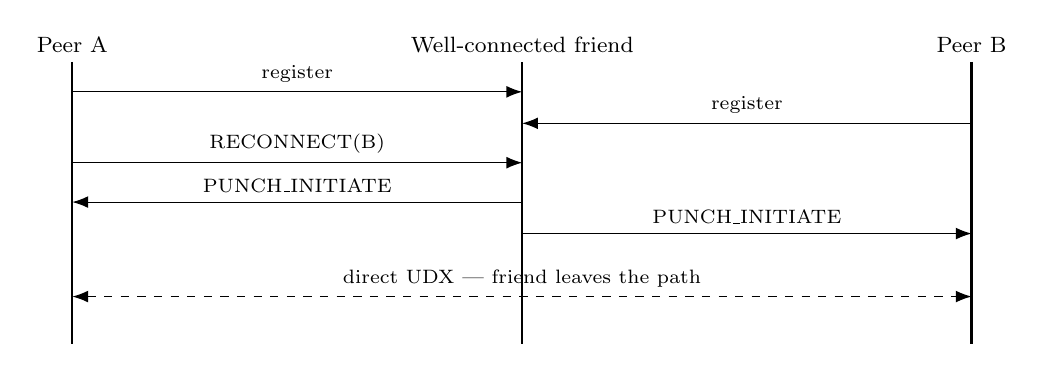
\begin{tikzpicture}[font=\footnotesize,>={Latex[length=2mm]}]
  \node (a) {Peer A};
  \node (f) [right=3.6cm of a] {Well-connected friend};
  \node (b) [right=3.6cm of f] {Peer B};
  \foreach \n in {a,f,b} \draw[thick] (\n) -- ++(0,-3.8);
  \draw[->] ($(a)+(0,-0.6)$) -- node[above,font=\scriptsize]{register} ($(f)+(0,-0.6)$);
  \draw[<-] ($(f)+(0,-1.0)$) -- node[above,font=\scriptsize]{register} ($(b)+(0,-1.0)$);
  \draw[->] ($(a)+(0,-1.5)$) -- node[above,font=\scriptsize]{RECONNECT(B)} ($(f)+(0,-1.5)$);
  \draw[<-] ($(a)+(0,-2.0)$) -- node[above,font=\scriptsize]{PUNCH\_INITIATE} ($(f)+(0,-2.0)$);
  \draw[->] ($(f)+(0,-2.4)$) -- node[above,font=\scriptsize]{PUNCH\_INITIATE} ($(b)+(0,-2.4)$);
  \draw[<->,dashed] ($(a)+(0,-3.2)$) -- node[above,font=\scriptsize]{direct UDX --- friend leaves the path} ($(b)+(0,-3.2)$);
\end{tikzpicture}
\caption{NAT hole-punch mediated by a well-connected friend. The friend relays only addresses and \code{PUNCH\_INITIATE}; the deterministic initiator (lexicographically smaller pubkey) then dials the direct UDX stream.}
\label{fig:holepunch}
\end{figure}


\section{Mesh Routing: Request-Driven Conveyance \& DTN Store-Carry-Forward}

The Bluetooth mesh is where Grassroots earns the word \emph{opportunistic}: a message reaches a friend who is not a direct neighbour by hopping across intermediaries, and a message for a friend who is momentarily out of range is carried until they reappear. Both behaviours live in one place. Every inbound packet, from every transport, enters the router through the single method \code{processPacket} (\code{lib/src/routing/message\_router.dart}). This is deliberate: BLE-arrived and UDP-arrived packets are demultiplexed by the same dispatch, deduplicated against the same seen-packetId set, and (for BLE) carried by the same rule, so there is exactly one definition of ``what happens to a packet.'' As established in \emph{Wire Format \& Packets}, the outer header the router sees is sender-anonymous — recipient ID, type, TTL, packet ID, and length only — so every decision below is made without knowing who originated the packet, and without being able to read its contents.

\subsection*{The dispatch: announce and handshake are special}

\code{processPacket} first peels off the two packet types that are \emph{not} mesh traffic. An \code{announce} is handed to the ANNOUNCE handler and returned early — never deduplicated, never relayed (\code{message\_router.dart}). A \code{noiseHandshake} is checked as addressed-to-us and dispatched, then likewise returned early (\code{message\_router.dart}). Both are minted with TTL 1 at the coordinator (\code{grassroots\_network.dart} for ANNOUNCE, \code{grassroots\_network.dart} for the handshake too), which makes them structurally \textbf{neighbour-local}: both are handled and returned \emph{before} the dedup-and-carry block below, so neither is ever deduplicated, taken into custody, or conveyed --- and their TTL of 1 means that even if one leaked into the carry path it would decrement to 0 and never be forwarded. The rationale is that both are about \emph{presence and pairwise key agreement}, not reach: ANNOUNCE advertises ``I am here, and here is my signed identity'' to immediate neighbours, and the Noise \code{XX} handshake — as detailed in \emph{The Noise Session Layer} — is today a neighbour-local exchange. A from-scratch multi-hop handshake (Noise \code{IK}/\code{KK} carried across relays) is \textbf{future work}; the current handshake reaches only direct neighbours, which is why an existing session, not a fresh handshake, is what lets a carried message reach a non-adjacent recipient.

\subsection*{Taking transit packets into custody}

Everything that survives the early returns — i.e.\ every \code{secure} envelope — is a mesh packet. The router deduplicates it by calling \code{checkAndAdd} on the outer \code{packet.packetId} against the seen-packetId set (\code{SeenPackets}, discussed below); \code{firstSeen} is the negation of ``was already present''. Before anything else, note the outermost branch: the whole carry block is nested inside \code{if (!forUs)}. A packet addressed to \emph{this} node is never carried no matter what its TTL says — it is deduplicated, trial-decrypted and delivered, and that is all. Carrying is what happens to \emph{other people's} traffic. Within that branch, a packet is taken into custody only when two conditions hold simultaneously:

\begin{enumerate}
\item \textbf{First sight.} \code{firstSeen} is true — a duplicate is dropped, killing loops and re-processing.
\item \textbf{TTL budget.} \code{packet.ttl > 0}. The node decrements the TTL once (\code{packet.decrementTtl()}) and takes the \emph{hopped} copy into custody, so the TTL falls by one per arrival and a packet arriving at~0 is not carried. A packet arriving at~1 is still taken in, held at~0 --- worth doing because the destination is exempt from this branch entirely, so a neighbour who is the recipient still accepts that last-hop copy when it is later conveyed. The default starting TTL is~7 (\code{packet.dart}), bounding any packet to at most seven hops of spread.
\end{enumerate}

Carrying is \textbf{open}: it is not friend-gated. The router takes a sealed packet into custody for a recipient it has no relationship with, because it can only see the recipient ID and opaque ciphertext — it cannot read the body, and the header carries no sender to authorise against. This is the deliberate reversal that gives the mesh its reach, and it is safe precisely because a carrier handles nothing but recipient-addressed sealed bytes.

Crucially, nothing is re-broadcast. The decremented, still-sealed packet is placed in the DTN store (below) and stays there; it leaves only when a neighbour's sync filter proves that neighbour lacks that packet ID, at which point the identical opaque ciphertext is conveyed to that one neighbour over its authenticated session --- BLE only, since UDP stays direct point-to-point per \emph{The Internet Transport}. A carrier \emph{cannot} re-seal, because it cannot decrypt; it copies opaque bytes. There is deliberately no push: a held packet is offered onward only in response to a request. This is distinct from the coordinator sending its \emph{own} traffic, which is not carrying at all. That path has two shapes: an addressed \code{send} goes through the router's \code{dispatchOutbound} (\code{message\_router.dart}), which direct-writes the sealed packet to the recipient if it is a connected neighbour and otherwise drops it into the same DTN buffer; and the coordinator's \code{broadcast(payload)} method seals a \emph{fresh} copy per neighbour under each peer's Noise session and airs them via \code{\_floodViaBle} (\code{grassroots\_network.dart}). Both send plaintext the coordinator itself holds --- the originator is simply the first node holding its own packets --- and neither is relaying.

For the same reason, a write to a peer --- whether a conveyance or a direct send --- puts each packet on exactly \textbf{one leg per peer}, preferring our peripheral leg --- a notification is unacknowledged at ATT level and several can pack into one connection interval, whereas the central leg writes to the peer's characteristic. Writing both legs put identical bytes on the air twice per neighbour and the receiver's seen-packetId set simply dropped the second copy. This was measured rather than reasoned about: a 500-message cycle-check run recorded exactly 1000 redundant packet arrivals --- a clean 2$\times$ --- before the change, and 0 after. The second leg is still maintained --- it is the pair's other direction, and it is now literally the redundancy on failure: when the chosen leg refuses a write, \code{\_writeToPeer} retries the same bytes on \code{otherLegFor}'s leg and logs a \code{retry} trace record for the save. This is not the double-send the one-leg rule forbids, because the fallback runs only after a throw and both platforms fail \emph{before} transmitting, so the packet cannot reach the air twice. The retry is gated on the other leg's own MTU (the two legs negotiate separately, and writing a packet that leg will truncate would put an unparseable write on the air and report success) and is skipped for a path whose identity is unknown, since without a pubkey there is no way to tell the pair's other leg from a stranger's.

\subsection*{The seen-packetId set}

Dedup is \emph{not} a Bloom filter. It is \code{SeenPackets} (\code{lib/src/mesh/seen\_packets.dart}): an \textbf{exact}, age-bounded set of packet IDs, keyed by the id, with no false positives and --- deliberately --- \textbf{no count cap and no hard-clear rotation}. Each entry keeps the packet's own \code{createdAtMs} (its originator-stamped creation time) alongside its first-seen time; entries are insertion-ordered by first-seen, and the set is pruned only by age, dropping any id older than \code{maxAge} = 6~hours (chosen to equal the DTN buffer's \code{maxAge}). The reasoning is precise: a copy of a packet can reach this node again only while some node still holds it, and a held packet leaves its buffer on ACK, on eviction, or at \code{DtnStore.maxAge} --- so a seen id must \emph{outlive} the buffer, after which re-admission is harmless because no copy can exist. This is a direct correction of the previous \code{BloomFilter}, which stayed bounded only by a \textbf{hard full clear} every 10{,}000 items or 5 minutes: under load that clear forgot everything, and a re-conveyed copy of a packet this node had already carried then looked new, so it was re-admitted, re-stored in the DTN buffer, and re-circulated. An exact set with no count cap cannot make that mistake, because it never evicts a live id. The same set is \emph{also} what a node advertises in the sync exchange --- as a GCS filter over a window of its seen ids (below) --- so ``what I have seen'' and ``do not resend me these'' are one structure. ANNOUNCE and handshakes never touch it at all, having returned early.

\subsection*{Bounding conveyance: TTL and dedup, and nothing else}

Open carrying needs a bound, and it has exactly two: a TTL that is decremented once per arrival and refuses to carry at~0, and the seen-packetId set, which admits any given packet at most once. Together they cap a packet's spread at seven hops and one conveyance per node per packet, which is a bound on the total work carrying can create --- not merely on its rate.

There used to be a third: a per-neighbour relay rate cap of 512 packets per 10-second window, refusing further relays on a neighbour's behalf until the window rolled over. It has been \textbf{deleted}. The case against it was measured, not argued: on \code{scf-check-4} it fired \code{relay / rateLimited} roughly 3{,}400 times across seven of eight phones, with \code{sync / budgetExhausted} at the top of the drop table --- at that rate the ceiling was shaping delivery on an ordinary eight-phone desk mesh rather than bounding an abuser. It also had two structural problems that made its headline number close to fiction. It was charged twice per packet for a period, because the predicate both tested and incremented and was evaluated in two arms of the same condition chain, so the effective ceiling was 256 rather than 512. And it was keyed by inbound path rather than peer identity, so a converged dual-leg pair held two independent budgets and every ${\sim}30$\,s MAC rotation minted a fresh allowance. Both were fixed before the cap was removed; what remained after the fixes was a limit that cost messages without adding a bound TTL and dedup did not already provide.

The consequence to state plainly: a node will now carry for a neighbour as fast as that neighbour can feed it, for as long as the packets are first sightings with TTL left. Carrying is still finite --- seven hops, once per node --- but its \emph{rate} is unbounded, and a neighbour that feeds it faster costs this node proportionally more radio and battery. Restoring a rate limit is therefore a live option if a future run shows a node being driven flat by one neighbour; what the measurement showed is that 512 per 10\,s was far below the level at which that becomes the problem.

\subsection*{The DTN memory buffer: one store for relays and senders alike}

There is no ``deliver now'' path for a carried packet, so \emph{every} transit packet that clears the two conditions above is cached --- not only the ones whose recipient happens to be out of range. With nothing pushing, a packet this node does not keep is a packet it can never offer onward: it would simply die here. So once a packet's TTL is decremented, the hopped, still-sealed copy is stored in the DTN store keyed by recipient hex (\code{message\_router.dart}), whether or not that recipient is currently reachable. The ordering still matters at the other end: a packet that could not be carried on arrival --- no TTL left, or already seen --- is not cached either, so nothing unforwardable ever reaches a buffer.

That cache is the \textbf{DTN memory buffer}: concretely \code{DtnStore.\_byRecipient}, a \code{Map<String, List<\_Entry>{}>} from recipient public-key hex to the sealed packets currently held for that recipient. It lives in memory and does not survive a process restart. A packet is in the buffer exactly while this node holds the sealed bytes and has not seen proof they arrived. It leaves by one of four routes: the recipient's end-to-end ACK (the only \emph{successful} exit, via \code{removeById}), age expiry, store-wide cap eviction, or recipient-cap eviction. The store fires a drop callback for the three non-ACK exits with a distinguishing reason (\code{expired}, \code{evictedTotal}, \code{evictedRecipients}), precisely so that a \code{custody store} trace record with no matching \code{end} is not ambiguous between ``still held'' and ``silently discarded'' --- which is exactly the packet-loss evidence the testbed needs. \textbf{The sender puts its own outgoing packets into that same buffer}, so a relay carrying a stranger's packet and a sender holding its own message are the same state in the same map, differing only in who wrote the entry.

The earlier design kept these apart, and the difference is concrete. Sending used to register each message in a table with a five-second timer; if the timer fired before an ACK, the message was pushed back onto a per-recipient outbound queue, which a periodic drain re-sent when the peer looked reachable. Relays, separately, kept the cache described above. Two mechanisms meant two answers to ``has this been delivered?'', which could disagree --- a message could sit in the sender's queue while a relay was already carrying a copy of it. The timer, the queue and the drain were deleted outright; the store-carry-forward mechanism itself did not change, and what remains is that one buffer with one exit condition. Confirmations follow the same rule: ACKs and read receipts are themselves sealed, put in their originator's buffer, and conveyed like any other recipient-addressed packet. Since nothing acknowledges an acknowledgement, a confirmation leaves the buffer only by age expiry.

\subsection*{The sync exchange, and why nothing is pushed}

Buffered packets move between nodes through exactly one mechanism: a sealed \emph{sync exchange} that runs when a pairing forms and on every later announce cycle. It is a single directed frame, not a round trip. A node advertises what it has \emph{seen} --- a \textbf{GCS (Golomb-coded set) compact filter} of packet IDs drawn from its \code{SeenPackets}, over a creation-time window --- and the peer answers by conveying, from its own DTN buffer, exactly the packets in that window whose IDs the filter proves it has \emph{not} seen (\code{buildSyncFilter}/\code{\_handleSyncFilter}, \code{message\_router.dart}). There is no separate offer-then-request handshake and no reply frame: the filter alone carries everything the responder needs, so a converged pair falls silent by construction --- once each side has seen the other's packets, every filter yields an empty difference and nothing is conveyed. The frame is a \code{SecureFrame} sealed to the pair's Noise session (\code{ContentType.syncFilter}, TTL~1, BLE only) --- the session already exists by the time sync runs, so there is no reason to put a summary of buffer contents on the air in the clear.

Two design choices in that filter are load-bearing. First, a node advertises what it has \emph{seen}, never what it currently \emph{holds}. A held-set filter says in effect ``I have nothing, send me everything,'' so a node that had already delivered a message and dropped it from its buffer would be re-sent the whole backlog --- measured at \textbf{12.76 conveyed copies per message} on the air. Because \code{SeenPackets} outlives the buffer, an emptied node still advertises ``I have seen these,'' and the responder conveys nothing it has already handed on. Second, the filter carries a creation-time \emph{window} \code{[fromMs, toMs]} (originator-stamped milliseconds), and the responder answers \emph{only} from packets whose own creation time falls inside it (\code{DtnStore.windowBetween}). This is what lets a single fixed-size filter advertise a slice of a large buffer without provoking a re-send of everything outside the slice: a filter that names a subset cannot be read as ``resend the rest.'' A node sweeps a cursor forward through its seen ids across successive rounds, oldest first, so the longest-waiting backlog is reconciled first and the whole buffer is covered over time. There is no decline ledger and no open-round bookkeeping --- nothing is inferred from silence, because there is no reply to be silent about.

The alternative --- sending the held packets themselves the moment a session forms, without asking --- was implemented, measured, and deleted. The flaw is that the holder cannot know what the peer already has; only the peer knows that. So it re-sent packets the peer had received, processed and discarded long before.

The cost of the blind push was measured over a 90-cycle overnight run. At \emph{every} reconnection the receiving phone re-sent \textbf{30.9 packets} the other side had already dealt with: 2784 wasted packets across the run. They were all acknowledgements --- the receiver had ACKed each message and kept its copy, and because nothing acknowledges an acknowledgement those copies never left the store, so the whole accumulated set went back on the air each time the link re-formed. At 187 bytes per ACK that is roughly 520\,KB out of 1686\,KB of acknowledgement traffic: \textbf{31\% of it was redundant}. Advertising identifiers instead of packets removes that, but an explicit id list is itself costly: a packet ID is a 16-byte UUID, so an id list fits only 8 per sealed write, and advertising a large buffer that way put real airtime on the wire for no payload --- a 17{,}116-packet buffer (measured peak, \code{scf-rearm-4}) cost about \textbf{2{,}140 packets}, and the id-list offer traffic was \textbf{46--51\%} of all sealed air across two runs. The GCS filter (\code{lib/src/mesh/gcs\_filter.dart}) replaces the id list wholesale: it costs about \code{p + 2} = 9 bits per element at \code{p = 7} --- a false-positive rate of \code{fprOneIn} = 1 in 128 (0.78\%) --- and is capped at \code{maxPayloadBytes} = 120 bytes, so one sealed filter advertises up to \code{maxElements} = 106 ids and the same 17{,}116-packet buffer fits in a few hundred bytes. A false positive merely withholds one packet for one round and self-heals as the window advances --- the same class of bounded miss the seen set already makes, and a fresh membership draw each cycle means no packet can stay invisible. A buffer larger than one filter advertises a subset per round, the cursor sweeping the rest over successive announce cycles.

Two consequences follow, both deliberate. First, the exchange is \textbf{BLE-only}: the Internet transport moves nothing out of the buffer --- not third-party traffic, not even packets held for the peer it is talking to --- because it stays strictly direct point-to-point. A buffered message is therefore redeliverable over BLE alone, so a friend reachable \emph{only} over the Internet does not receive it until a BLE encounter or age expiry. Direct sends over UDP are unaffected; the buffer exists precisely for recipients who were unreachable at send time. Second, because reconciliation is driven by the peer's seen-set rather than by the holder's guess, the mesh's replication is genuinely epidemic: any node that meets any other converges toward carrying what the other lacks.

\subsection*{Bounding every buffer}

The store (\code{lib/src/mesh/dtn\_store.dart}) is bounded on three axes:

\begin{itemize}
\item \textbf{Age.} Entries older than \code{maxAge} = 6~hours are pruned on every access.
\item \textbf{Total bytes.} At most \code{maxBytes} = \textbf{512\,MiB} of sealed payload across all recipients, evicting the globally-oldest packet until the store is back inside the ceiling. The bound is \emph{bytes}, not a packet count: a count says nothing about memory unless every packet is the same size, and a fragmented message is several packets of whatever the MTU left over. (It counts sealed payload bytes, not the Dart object overhead around each entry, so real process memory sits somewhat above the figure --- on a 2\,GB handset the per-app heap limit is reached first and the OOM killer becomes the effective bound.) This store-wide byte bound replaced an earlier per-recipient depth of 32, which had two faults: it silently dropped a busy peer's oldest undelivered packets while the rest of the buffer sat empty, and --- because confirmations only age out --- it pinned a full 32 held acknowledgements per peer, which is what made the blind push cost exactly that much.
\item \textbf{Recipient count.} At most \code{maxRecipients} = 256 distinct recipients; when exceeded, the store evicts the recipient whose oldest packet is oldest.
\end{itemize}

The bound applies to every buffer on the message path, not just the sealed store --- and the strongest bound is the one on what never exists: there is \emph{no pre-seal hold}. A send to a peer without a Noise session fails immediately, so no plaintext payload is ever buffered on behalf of a peer that might never appear (see \emph{Sending a Message}). The \textbf{packet-ID index}, which maps a message to the buffered packets to release when its ACK arrives, is bounded by the buffer itself: the DTN store reports \emph{every} non-ACK exit (age expiry and both evictions) through an \code{onDrop} callback, and the coordinator releases the corresponding index entry on that signal as well as on ACK --- so an entry cannot outlive the packets it points at. A fixed \code{\_maxAckIndexEntries} = \textbf{200{,}000} backstop guards against a runaway. Sizing this wrong once broke exactly that mechanism: an earlier bound of 1000, borrowed from \code{MessagesState.maxMessages} (an unrelated UI-history depth), filled almost immediately at the saturation rate, and because it then evicted \emph{live} entries it silently turned ACK-driven buffer release off --- a 7-device smoke run evicted 178{,}138 index entries and left packets held until they aged out. Capping the sealed buffer while an unsealed one in front of it grows without limit merely moves the leak upstream --- and sizing a cap against the wrong quantity breaks the mechanism it was meant to protect.

\subsection*{Two distinct dedup keys, and what a duplicate triggers}

Because a large message is fragmented, the router keeps two separate dedup domains. Relay and loop suppression run on the \textbf{outer} \code{packetId} (pre-decrypt), so an intermediary dedups without reading anything. Message \emph{delivery} dedup runs on the \textbf{inner} \code{messageId} recovered from the reassembled \code{SecureFrame} after decryption. A first-seen fragment is therefore relayed, while the application receives the assembled message exactly once.

What happens to a duplicate that still arrives is a rule worth stating explicitly, because the obvious alternative is wrong: \textbf{a duplicate of an already-delivered message triggers nothing.} No re-delivery, and no re-acknowledgement. An earlier design re-ACKed duplicates on the theory that a lost ACK deserves a second chance; the effect was that every redundant copy on the air generated a redundant confirmation back, and a sender whose ACK was genuinely lost is already covered --- it still holds the message in its buffer, and the next sync exchange reconciles it. Dedup means drop.

The two namespaces must never be joined. They are equal only for unfragmented messages, where \code{packetId} is set equal to \code{messageId}; every fragment carries a random \code{packetId}. Joining a packet-level duplicate count against message-level records once produced a plausible-looking ``3.35$\times$ duplication factor'' that was pure nonsense, since the two id spaces share no values by construction.

\section{The Noise Session Layer}

Every end-to-end guarantee in Grassroots rests on a single component: a hand-rolled implementation of the Noise Protocol Framework's \code{XX} handshake, living in \code{lib/src/session/noise\_session\_manager.dart}. The transport deliberately owns this code rather than deferring to a black-box library, because the mesh imposes requirements a generic Noise library does not anticipate: sessions must be demultiplexed without a sender field on the wire, they must survive a peer moving between relay paths and transports, and the transport-message AEAD must bind exactly those envelope fields a relay may \emph{not} mutate. This section explains how the layer meets those requirements, and marks clearly where today's implementation is neighbour-local and a broader design remains future work.

\subsection*{Pattern, roles, and the three-message handshake}

The concrete protocol is \code{Noise\_XX\_25519\_ChaChaPoly\_SHA256} (\code{noise\_session\_manager.dart}): the \code{XX} handshake pattern, X25519 Diffie--Hellman, ChaCha20-Poly1305 for authenticated encryption, and SHA-256 for hashing. \code{XX} is a mutual-authentication pattern in which neither party knows the other's static key in advance --- both static keys are transmitted, encrypted, \emph{during} the handshake. This matches the mesh's trust model, where a node may cold-call a neighbour it has never spoken to.

The handshake is exactly three messages, enumerated \code{message1(1)}, \code{message2(2)}, \code{message3(3)} (\code{noise\_session\_manager.dart}), exchanged between an \code{initiator} and a \code{responder} (\code{NoiseHandshakeRole}). The initiator writes messages 1 and 3; the responder writes message 2. Each message has a fixed, strictly-checked size, so a malformed handshake fails fast rather than degrading:

\begin{itemize}
  \item \textbf{Message 1} --- 32 bytes: the initiator's ephemeral X25519 public key, sent in the clear (\code{noise\_session\_manager.dart}).
  \item \textbf{Message 2} --- 80 bytes: the responder's ephemeral (32 bytes) plus its encrypted static key (32-byte key + 16-byte MAC = 48 bytes) (\code{noise\_session\_manager.dart}).
  \item \textbf{Message 3} --- 48 bytes: the initiator's encrypted static key (32 + 16) (\code{noise\_session\_manager.dart}).
\end{itemize}

Each handshake message is wrapped in a small versioned frame, \code{[version=1][message-value][body]} (\code{noise\_session\_manager.dart}), and a decode of fewer than two bytes or a wrong version byte is rejected --- there is no tolerance for a truncated or older frame, in keeping with the project's no-compatibility-shim rule.

\subsection*{Symmetric-state primitives}

The manager implements the Noise symmetric-state machine directly (\code{noise\_session\_manager.dart}). \code{initialize} seeds a 32-byte hash from the protocol name; \code{mixHash} folds new data into that running transcript hash as $\text{SHA-256}(\text{hash}\,\|\,\text{data})$; and \code{mixKey} runs a two-output HKDF-SHA256 (\code{\_hkdf2}) to derive a fresh chaining key and cipher key, resetting the per-key nonce to zero. \code{encryptAndHash} / \code{decryptAndHash} apply ChaCha20-Poly1305 using the current transcript hash as AAD, so every ciphertext is bound to everything exchanged so far. A subtle but correct detail is the \textbf{pre-first-\code{mixKey} passthrough branch}: while no cipher key exists yet (\code{cipherKey == null}), \code{encryptAndHash}/\code{decryptAndHash} pass their data through as cleartext and merely \code{mixHash} it, so the symmetric state behaves correctly before any key material exists. Message~1 does not actually travel that path --- \code{writeMessage1} generates the ephemeral, calls \code{mixHash} on it directly and returns the raw bytes --- but it travels unencrypted for the same reason, that \code{XX} has no key material yet at that point, and it is authenticated retroactively by the transcript. Finally, \code{split} derives the two directional transport keys from an HKDF-2 over the final chaining key, with the initiator's send/receive keys being the responder's receive/send keys, giving each direction its own key.

\subsection*{Identity inside the handshake, and the birational check}

Grassroots identity is an Ed25519 key pair, but Noise operates over X25519. The manager bridges the two with libsodium's birational map: the local Noise static is derived from the Ed25519 identity via \code{skToCurve25519}/\code{pkToCurve25519} (\code{noise\_session\_manager.dart}). It is worth being exact about what travels where, because the loose phrasing ``the identity is conveyed inside the handshake'' is common and slightly wrong. What the encrypted handshake carries is the peer's \emph{X25519 static key}, per the \code{XX} pattern. The peer's \emph{Ed25519 identity} is never on the wire in this exchange at all --- neither in a cleartext header nor inside the ciphertext. It is resolved out of band by the coordinator, from the inbound path: on BLE from the neighbour's verified self-signed ANNOUNCE, on UDP from the peer id (which is the pubkey hex). The manager receives it as the \code{remotePubkey} argument to \code{handleHandshakePacket}. To prevent a peer from presenting a Noise static that does not correspond to that identity, \code{\_verifyRemoteStatic} recomputes \code{pkToCurve25519(remotePubkey)} and compares it, in constant time (\code{\_bytesEqual}), against the static Noise actually delivered. The binding therefore runs between an out-of-band, ANNOUNCE-authenticated identity and an in-band, encrypted static. If they disagree --- or the point is invalid --- verification fails and no session is formed. This is the load-bearing authentication check: there is \textbf{no per-packet Ed25519 signature} anywhere in this layer, correcting a stale class-doc remark that lists ``signing packets'' as a use of the identity (\code{identity.dart}); only ANNOUNCE is payload-signed, and the identity's private key is used here purely for this static-key derivation.

\subsection*{Keying by peer, and sender-anonymous demultiplexing}

Sessions are stored in a map keyed by the peer's Ed25519 public key rendered as hex (\code{noise\_session\_manager.dart}, \code{\_hex}) --- \emph{not} by transport path or socket. A session therefore transparently survives a peer switching relay paths on the BLE mesh or moving between BLE and Internet transports; the same key material serves every path. Because the outer envelope is sender-anonymous (recipient-only, no sender field), an inbound \code{secure} packet carries nothing that says which session decrypts it. The manager resolves this by \textbf{trial-decrypt} (\code{trialDecrypt}): it attempts an AEAD open against the active sessions, walking the table \emph{most-recently-used first} --- the order \code{\_touch} maintains by re-inserting an entry on every send and every successful decrypt --- and stopping at the first that opens; the Poly1305 tag succeeds for at most one session, which both selects the session and recovers the sender's identity as a by-product. The call returns the cleartext packet together with the recovered sender pubkey, or \code{null} if no session matches. On the send side, \code{encryptPacket} seals only \code{secure}-typed packets and leaves the type as \code{secure} (the post-refactor design no longer swaps in ``secure-variant'' packet types), so relays observe an identical opaque type for every content class.

\subsection*{Transport AEAD, AAD, and replay}

An encrypted transport payload is laid out as \code{[version=1][8-byte little-endian nonce][ciphertext $\|$ 16-byte MAC]} (\code{noise\_session\_manager.dart}), the 64-bit counter being written little-endian at offset~4 of a 12-byte ChaCha20-Poly1305 nonce buffer (\code{\_aeadNonce}). The associated data (AAD) is 81 bytes: the constant \code{secure} wire type (1) $+$ sender pubkey (32) $+$ recipient (32) $+$ packetId (16) (\code{\_applicationAad}). It \textbf{deliberately excludes \code{ttl}}, precisely because a relay decrements TTL in flight --- binding TTL would break end-to-end authentication the moment the packet was forwarded. TTL is now the \emph{only} meaningful header field left unbound: the 4-byte header timestamp that earlier editions listed alongside it no longer exists on the wire at all, and the one other unbound field, the payload length, is purely the stream framer --- tampering with it truncates the ciphertext and the AEAD tag fails anyway. The content type is \emph{not} in the AAD because it no longer lives on the wire at all; it sits inside the AEAD-protected plaintext as a \code{SecureFrame}, and is thus authenticated by the ciphertext itself (see \emph{The Wire Protocol}). Replay is resisted per direction by a bounded set of received nonces capped at 2048 with FIFO eviction; a duplicate nonce raises a \code{StateError}. This is a \emph{bounded} guard, not an absolute one --- a nonce evicted after 2048 newer arrivals could in principle be replayed --- a documented trade-off between memory and strictness.

\subsection*{Establishment scope, timeouts, and future work}

Handshake liveness is enforced twice, because the two failure modes are different. A caller that is waiting gets a 5-second timeout on \code{waitForSession} --- the manager's default \code{handshakeTimeout} --- and on expiry the half-built entry is dropped, a \code{drop} record with reason \code{timeout} is traced, and \code{false} is returned. A handshake that \emph{nobody} is awaiting is caught by the second mechanism: \code{\_reapDeadHandshakes}, run each time a session is established, removes every entry older than twice the handshake timeout that holds no session, releasing any waiter with \code{false}. Without it a peer that vanishes after message~1 would leave its entry behind for the life of the process, since nothing else removes a handshake no caller is blocked on. Simultaneous initiation --- both peers sending message~1 at once --- is broken deterministically by comparing local and remote pubkey hex: the lexicographically-smaller side keeps its initiator handshake and ignores the inbound message~1, the other abandons and becomes responder.

Today, handshake establishment is strictly \textbf{neighbour-local}: both ANNOUNCE and \code{noiseHandshake} packets are sent with \code{ttl: 1} and are never relayed, and \code{remotePubkey} is resolved by the coordinator from the neighbour's verified self-signed ANNOUNCE on the inbound BLE path rather than from the packet (which carries no sender) (\code{noise\_session\_manager.dart}). A session, once formed, is end-to-end and survives relaying --- but forming one requires the two endpoints to be direct neighbours. A from-scratch multi-hop handshake using the \code{IK}/\code{KK} Noise patterns, which would let two non-adjacent mesh nodes establish a session across relays, is \textbf{future work} and is not implemented.


\begin{figure}[htbp]\centering
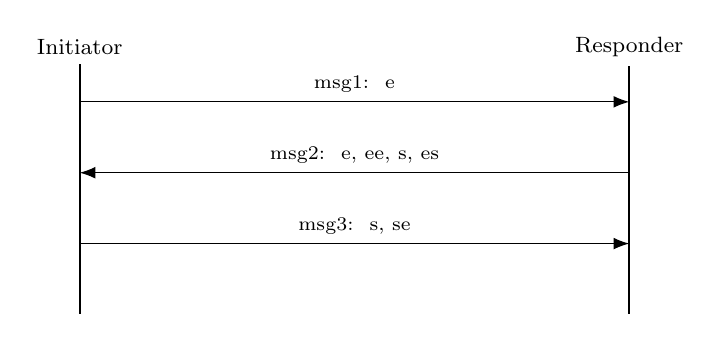
\begin{tikzpicture}[font=\footnotesize,>={Latex[length=2mm]}]
  \node (a) {Initiator};
  \node (b) [right=5.5cm of a] {Responder};
  \draw[thick] (a) -- ++(0,-3.4);
  \draw[thick] (b) -- ++(0,-3.4);
  \draw[->] ($(a)+(0,-0.7)$) -- node[above,font=\scriptsize]{msg1:\; e} ($(b)+(0,-0.7)$);
  \draw[<-] ($(a)+(0,-1.6)$) -- node[above,font=\scriptsize]{msg2:\; e, ee, s, es} ($(b)+(0,-1.6)$);
  \draw[->] ($(a)+(0,-2.5)$) -- node[above,font=\scriptsize]{msg3:\; s, se} ($(b)+(0,-2.5)$);
\end{tikzpicture}
\caption{The \code{Noise\_XX\_25519\_ChaChaPoly\_SHA256} handshake. Static keys are transmitted encrypted; each side's Ed25519 identity is cross-checked against its Noise static via the birational map. Establishment is neighbour-local (handshake packets carry TTL 1).}
\label{fig:handshake}
\end{figure}


\section{State Management: the Redux Projection}

All shared state in the transport lives in a single immutable Redux store. The root of that store is \code{AppState}, an immutable value composed of exactly six slices (\code{lib/src/store/app_state.dart}): \code{transports}, \code{peers}, \code{messages}, \code{friendships}, \code{settings}, and \code{signaling}. The user interface reads from these slices and rebuilds when they change; the transport layers never mutate application state directly. Instead, every observable event flows through the Redux cycle: a transport observation is turned into an \emph{action}, a pure \emph{reducer} folds that action into a new immutable state, and \emph{subscribers} (the UI, the persistence service) react to the resulting change. This chapter's discussion of \emph{the coordinator} and \emph{the Noise session layer} describes the producers of these actions; here we describe where their facts land and how they are shaped.

\subsection{The six slices}

Each slice owns one concern and nothing more.

\begin{itemize}
  \item \textbf{PeersState} (\code{lib/src/store/peers_state.dart}) holds \code{discoveredBlePeers} (raw BLE discoveries keyed by radio path id), \code{peers} (identified peers keyed by public-key hex), and a \code{friendsOfFriends} adjacency map. A \code{PeerState} records both BLE legs of the mandatory dual-role pair as two separate path-id fields (\code{bleCentralDeviceId}, \code{blePeripheralDeviceId}), the peer's UDP address plus a set of advertised \code{udpAddressCandidates} and a link-local fallback, and derived predicates such as \code{isReachable}, \code{hasBleConnection}, \code{activeTransport}, and \code{isWellConnected}.
  \item \textbf{MessagesState} (\code{lib/src/store/messages_state.dart}) holds delivery-status records (\code{outgoingMessages}/\code{incomingMessages} keyed by message id), per-conversation chat history (\code{conversations} keyed by peer hex, oldest first), and \code{unreadCounts}. It is bounded: \code{maxMessages}$=1000$ and \code{maxMessagesPerConversation}$=500$. Notably this slice carries application-level chat and even view-once picture media as first-class content, which sits a little above the ``pure packet transport'' framing of the rest of the system.
  \item \textbf{FriendshipsState} (\code{lib/src/store/friendships_state.dart}) is a map keyed by \code{peerPubkeyHex}; each entry carries \code{status} (\code{pending}, \code{received}, \code{accepted}, \code{declined}), the friend's last-known \code{udpAddress}, a \code{nickname}, \code{createdAt}/\code{updatedAt}, and an optional request \code{message}. (The \code{knownRvServers} map earlier editions listed here is gone, deleted with the rendezvous servers.) Receiving a friend request while our own request to the same peer is outstanding auto-accepts, giving a mutual-request handshake.
  \item \textbf{TransportsState} (\code{lib/src/store/transports_state.dart}) tracks the two transports' lifecycles \emph{independently} through separate \code{bleState} and \code{udpState} fields (plus per-transport error strings), our discovered \code{publicAddress}, and the current \code{networkConnectionType}. It also holds \code{bleScanning}, \code{publicIp} (the address without a port, retained even behind NAT), \code{publicAddressDiscoveryFailed}, the debug-only \code{bleLinks} --- the plugin's OS-level snapshot of live physical BLE links, empty unless \code{showLinkDiagnostics} has the poll running --- and \code{lastUnsolicitedInboundAt} --- the timestamp of the most recent unsolicited inbound datagram, which is the evidence that our mapping is externally reachable. ``Well-connected'' is defined here: \code{isWellConnected} is true iff we hold a globally routable public address.
  \item \textbf{SettingsState} (\code{lib/src/store/settings_state.dart}) holds the user-toggleable configuration: \code{bluetoothEnabled} and \code{udpEnabled} (both default true), \code{transportPriority} (default $[\text{bluetooth},\text{udp}]$), \code{coldCallTrustLevel} (default \code{open} --- see \emph{Cold-call trust}), \code{facilitateInvites} (default false, and AND-ed with the cold-call level before a node will broker for a stranger), the debug \code{bleRoleMode} and \code{showLinkDiagnostics}, and the testbed-only \code{bulkFlowConfig} (null and inert outside an experiment).
  \item \textbf{SignalingState} (\code{lib/src/store/signaling_state.dart}) is deliberately minimal: a single \code{holePunchAttempts} map from target peer hex to a \code{HolePunchStatus} (\code{requested}, \code{punching}, \code{succeeded}, \code{failed}). Hole-punch coordinates (ip, port, failure reason) ride \emph{on the actions} but are not retained in state --- only the status transition is recorded.
\end{itemize}

\subsection{The actions {\textrightarrow} reducers {\textrightarrow} subscribers cycle}

\code{appReducer} (\code{lib/src/store/reducers.dart}) is the root reducer. It dispatches by the action's base type --- \code{PeerAction}, \code{MessageAction}, \code{FriendshipAction}, \code{SettingsAction}, \code{TransportAction}, \code{SignalingAction} --- to the matching slice reducer, and returns the state unchanged for any action it does not recognise. Each slice reducer is a pure function of (old slice, action) $\rightarrow$ new slice, and \code{AppState.copyWith} threads the one changed slice into a fresh root. Because the state is immutable, subscribers detect change by value equality; a slice that a reducer leaves untouched is returned identically and triggers no rebuild.

\subsection{The strict-projection principle}

The governing rule is that the Redux state is a \emph{strict projection} of facts the transport layers explicitly emit --- never an inference. The rule binds \emph{reducers}: a reducer must not synthesise state from ``I have not heard from peer $X$ in $N$ seconds'' heuristics. \code{StalePeersRemovedAction} shows the discipline --- it only \emph{removes} non-friend peers past a staleness threshold and explicitly refuses to touch \code{connectionState}, because that field is driven solely by BLE plugin and UDX events (\code{lib/src/store/peers_reducer.dart}); friends are never removed at all.

Where timeout reasoning does live is one layer up, and it is worth being exact rather than claiming the system contains no such timer. A UDP disconnect drops reachability immediately when an explicit disconnect event arrives --- that is the primary path. \emph{In addition}, the coordinator runs a periodic stale sweep: \code{computeStaleUdpPeerPubkeys} flags any UDP-connected peer whose \code{lastUdpSeen} is older than twice the announce interval, and \code{_removeStalePeers} acts on the result (\code{lib/src/grassroots_network.dart}). That is a silence-based inference, deliberately sited in the coordinator --- which owns transport facts and may derive from them --- rather than in a reducer, which may not. The invariant constrains \emph{who} may infer; it does not claim that nothing anywhere reasons from silence.

\subsection{Transport independence and consolidated reachability}

The two transports are independent: losing or disabling one must have zero effect on the other. This invariant is encoded directly in the reducers. \code{PeerBleDisconnectedAction} preserves \code{hasLiveUdpConnection}, and \code{PeerUdpDisconnectedAction} preserves both \code{bleAuthenticated} and the stored \code{udpAddress} (kept for later reconnection) (\code{lib/src/store/peers_reducer.dart}). The two disconnect reducers are not symmetric about \code{connectionState}, and the asymmetry is worth knowing: \code{PeerUdpDisconnectedAction} gates the flip on the other transport (it keeps the existing \code{connectionState} when \code{hasBleConnection} is still true), whereas \code{PeerBleDisconnectedAction} does not condition on a live UDP link in the same way. Reachability itself is unaffected either way, because it is computed from the two authenticated-link flags rather than from \code{connectionState}: \code{isReachable} is exactly \code{bleAuthenticated} $\lor$ \code{hasLiveUdpConnection} (\code{lib/src/store/peers_state.dart}), with no branch, flag or peer-kind test of any sort. So a raw BLE or UDX link without a completed Noise session does not count as reachable, and --- unlike in earlier editions of this chapter --- there is \emph{no} rendezvous-server exception, because there are no rendezvous servers.

Application-level connectivity is reported as \emph{consolidated} end-to-end reachability rather than per-transport events. The coordinator's reachability diff (\code{processReachabilityTransitions}, \code{lib/src/grassroots_network.dart}) compares each peer's current \code{isReachable} against the previous tick and fires \code{onPeerConnected}/\code{onPeerDisconnected} only on a transition. Because reachability is the OR of the two transports, one of two live transports flipping leaves the OR unchanged and fires nothing --- a disconnect fires only when the \emph{last} transport drops (a $0 \leftrightarrow N$ live-transport transition). A peer removed from the map while still reachable is surfaced as a synthesised disconnect carrying only the reconstructed identity.

\subsection{The TransportState lifecycle}

Each transport moves through a six-state lifecycle enum (\code{lib/src/transport/transport_service.dart}): \code{uninitialized} $\rightarrow$ \code{initializing} $\rightarrow$ \code{ready} $\rightarrow$ \code{active}, plus \code{error} and \code{disposed}. A transport is ``usable'' when it is \code{ready} or \code{active}. \code{TransportsState} carries one such enum per transport (defaulting to \code{uninitialized}) so BLE and UDP progress through their lifecycles wholly independently.

\subsection{Selective persistence}

Persistence is deliberately partial. \code{PersistenceService} (\code{lib/src/store/persistence_service.dart}) writes exactly three domains to \code{SharedPreferences}: friendships, settings, and conversations-plus-unread-counts (under \code{v2}-versioned keys), debounced by a $500$\,ms timer with a \code{flush()} for app exit. The \code{peers}, \code{transports}, and \code{signaling} slices are \emph{intentionally not persisted}. This is the strict-projection principle applied to durability: peer, transport, and hole-punch state are live facts that must be re-derived from the transports at runtime, so restoring a stale snapshot of them would violate the projection. Friendships, user settings, and chat history, by contrast, are durable user data with no live source to re-derive from.

\subsection{The coordinator as the bridge}

\code{GrassrootsNetwork} (\code{lib/src/grassroots_network.dart}) is the bridge between the transports and the store. It subscribes to raw BLE and UDX events and to the Noise session layer, and translates them into actions. A completed Noise handshake becomes a \code{PeerBleAuthenticatedAction} or a \code{PeerUdpConnectionChangedAction(connected:\,true)}; a torn-down UDX session becomes the corresponding \code{connected:\,false}; an ANNOUNCE becomes address and peer-list updates. This is precisely where explicit transport facts enter the projection, keeping reducers free of any inference.

\subsection{Honest warts}

A few rough edges are worth recording. \code{lib/src/store/store.dart} is only a library barrel of export directives, not the actual store construction --- the store and middleware are wired elsewhere. \code{AppAction} (\code{lib/src/store/actions.dart}) is a dead abstract base class: none of the per-slice action base classes extend it, and \code{appReducer} takes a \code{dynamic action}, so it is orphaned. Several \code{hashCode} implementations are intentionally weak: \code{MessagesState}, \code{FriendshipsState}, and \code{SignalingState} all hash only the \emph{length} of their maps, so two structurally different states of equal size collide (equality via \code{==} remains content-exact). \code{PeerState}'s equality deliberately excludes \code{bleAuthenticated}, which means a change to that flag alone is invisible to Redux equality even though \code{isReachable} depends on it --- a latent missed-rebuild risk for reachability-driven UI. Finally, the debug log is a scoped exception to the ``no mutable singletons'' rule: \code{DebugLogScreen} and its \code{LogBuffer} bypass Redux entirely and keep their ring buffer in a mutable global singleton, unlike all other UI state, which reads \code{AppState}.

\section{Instrumentation: Tracing, Testbed Harnesses, and the Trace Server}

Several claims in this chapter are numbers --- 350\,\textmu s per failed AEAD open, 30.9 redundant packets per reconnection, 34--57 messages per second on a saturated link. They are not estimates, and the machinery that produces them is a real part of the tree rather than a scratch script, so it belongs in an architecture overview even though none of it runs in production. Two rules govern all of it: every entry point is inert unless an experiment is active, and nothing leaves the device without an explicit human action.

\subsection{In-app tracing}

\code{ExperimentRecorder} (\code{lib/src/trace/experiment_recorder.dart}) is the sink every other component logs to. While an experiment is active each record is buffered \emph{in memory} and appended to a per-experiment JSONL file only at boundaries deliberately placed outside a measurement window: the run's stop, each field-run step boundary (\code{FieldRunner} calls \code{flush()} between windows, never inside one), any share or upload that reads the files, and --- on a long discharge run --- every \code{flushEverySocDrop} $=5$ percentage points the state of charge falls; when no experiment is active, \code{log} is a no-op. The buffering is deliberate and the trade is explicit: no disk I/O happens inside a measurement window, because writing costs power and CPU and a \emph{timer}-paced flush would land its largest write inside the busiest condition --- biasing exactly what a power ladder measures. Pacing that discharge-run flush on state of charge rather than on a timer is what keeps it out of the measurement: the write rate follows the run's own progress --- roughly twenty small writes across a full discharge --- instead of scaling with traffic, and it exists because a discharge run has no clean stop to write at, the phone reaching its battery floor while still recording. The residual cost is that an app kill loses whatever accumulated since the last flush. Files leave the device only by the experimenter's own doing --- the share sheet, the manual upload button, or the upload that terminates a scripted field run they started --- and only in a build carrying a baked-in \code{TraceConfig} token; there is no background upload and no pseudonymisation, since records carry real pubkey hex so that runs correlate across devices offline.

The records are what make the mesh legible after the fact. A \code{relay} record carries the packet id, TTL in and out, hop number, the neighbour it came \emph{from}, whether the packet entered the DTN buffer, and \code{dwellMs} --- the receipt-to-forward time on \emph{one} clock. That last field is the design point: end-to-end latency decomposes into per-hop dwells plus carry times plus radio time, so it can be reconstructed without ever synchronising clocks between devices. Note also what a relay record deliberately omits: the recipient. A relay must not need one, and paths reconstruct by packet id alone, while the endpoints log recipient and message id --- so an offline join still recovers who a message was for without the mesh having carried that fact.

\code{WireLedger} (\code{lib/src/trace/wire_ledger.dart}) complements this with byte accounting, classifying every serialized packet by its outer type byte --- read off \code{GrassrootsPacket.packetIdOffset} rather than hardcoded, after a hardcoded byte range silently followed the old 58-byte header for one commit and, since any 16 bytes format as a UUID, returned an id that matched nothing instead of throwing --- and emitting periodic tx/rx deltas. It is what separates control-plane cost (ANNOUNCE plus handshake) from \code{secure} traffic; on the \emph{tx} side it splits \code{secure} further by the inner content type only the sender knows (\code{secure:data}, \code{secure:ack}, \code{secure:sync}), while rx \code{secure} stays aggregate --- which is precisely the distinction a peer on the air can make. Its monotonic \code{totalBytes} doubles as the field runner's dead-radio check: a segment that claims the radio is on and moves zero bytes is a radio that never came back up --- and it counts bytes \emph{on the air}, so a broadcast over $N$ links counts $N$ times.

\subsection{Testbed harnesses}

\code{lib/src/testbed/} holds the drivers, all gated behind debug settings that are null and inert by default. \code{BulkFlowDriver} generates sustained load for throughput arms; \code{CryptoBench} times the AEAD and handshake primitives on the device itself rather than inferring them from a laptop, which is what makes the \emph{cost of recipient anonymity} argument binding on 2015 hardware; \code{FieldRunner} and \code{FieldPlanPresets} sequence a scripted field experiment through placement, positioning, dwell, settle and finish phases. \code{TestbedConfig} sizes the default synthetic payload to \code{FragmentHandler.fragmentThreshold} (136 bytes) precisely so that one message is one packet and delivery ratios read per-packet with no hidden fragment multiplier.

The testbed no longer touches the wire at all. A field run starts only by the wall-clock-anchored manual launch: every phone is tapped individually, and each rounds up to the same alignment boundary, so the fleet begins on one shared instant and the start skew collapses to clock-sync error rather than the walk between phones. Two \code{ContentType} values (\code{0x07} \code{testbedStart}, \code{0x08} \code{testbedNeighbours}) once carried a broadcast start signal and an armed-time neighbour gossip for this subsystem; both are deleted, and their values retired, precisely because the wall-clock anchor made a radio-borne start --- and the pre-start connectivity check it needed --- redundant, and control traffic on the air is something a measurement is better off without.

\subsection{Off-device analysis}

\code{trace_server/} receives uploaded runs and analyses them: \code{analyze.py} (including the \code{session_cap()} sizing pass cited in \emph{Known limitations}), \code{contact_trace.py} for re-encounter distributions, \code{establishment_time.py}, and a topology viewer. \code{tools/} carries the fleet-operations scripts --- clock synchronisation across phones, deployment, packet decoding. The experiments themselves, their protocols and their results are documented separately in \code{docs/testbed_experiments.md}; this section exists only to place the in-app machinery in the architecture, and defers to that document rather than duplicating it.

\section{End-to-End Interaction Walkthroughs}

The preceding sections dissected the transport component by component. This
section reassembles them into six concrete narratives that trace a single
event as it flows across the layers. Each walkthrough is deliberately
step-by-step and cites the responsible component by file and symbol; the reader
should treat these as the ``integration tests in prose'' that show how the
sender-anonymous envelope, the Noise session layer, the request-driven conveyance mesh,
and the Redux projection actually cooperate at run time.

\subsection{Sending a Message}

A host application calls
\code{GrassrootsNetwork.send(recipientPubkey, payload)}
(\code{lib/src/grassroots\_network.dart}). The coordinator drives the following
sequence.

\begin{enumerate}
  \item \emph{Validate and identify.} \code{send} rejects any recipient public
    key that is not exactly 32 bytes, returning \code{null}. Otherwise it mints
    a v4 UUID as the \code{messageId} (if the caller did not supply one) and
    sets the wire \code{packetId} equal to it, so that the recipient's ACK ---
    which echoes the \code{packetId} --- correlates back to this send.
  \item \emph{Choose a transport, BLE first.} \code{\_trySendMessageNow}
    attempts the BLE mesh first and only falls back to the Internet transport
    when BLE is unavailable, honouring the ``BLE preferred'' rule.
  \item \emph{Ensure a Noise session.} The BLE send path is gated on holding a
    Noise session with the recipient. \code{\_ensureNoiseSession} completes an
    XX handshake only for a \emph{direct} neighbour (see below), but an
    \emph{already-established} session lets even a non-adjacent recipient be
    addressed, because sessions are keyed by peer identity, not by path.
  \item \emph{Seal the payload.} The message is wrapped in a
    \code{secure} packet whose plaintext is a \code{SecureFrame}
    (\code{lib/src/models/secure\_frame.dart}) carrying
    \code{contentType = message}; \code{NoiseSessionManager.encryptPacket} seals
    it to the recipient's session. The sender-anonymous envelope carries
    \emph{no} wire signature --- authentication is end-to-end inside Noise.
  \item \emph{Direct-write or buffer.} Over BLE the router's
    \code{dispatchOutbound} writes the sealed packet straight to the recipient
    when it is a connected neighbour, and otherwise holds it in the DTN buffer
    for the sync exchange to convey later --- there is no flood to \emph{all}
    neighbours. Over the Internet, the copy is a \emph{direct}
    point-to-point UDX write: an existing connection is reused, else the
    coordinator connects on demand to a known address, else it discovers the
    peer through a facilitator (walkthrough~5).
  \item \emph{Buffer them.} Any of those sealed packets not written directly go
    into the sender's own DTN memory buffer, keyed by recipient; every packet's
    ID is indexed under the \code{messageId} so a later ACK can release the
    buffered copies --- the sender holds its own undelivered packets exactly as a
    carrier would hold a stranger's. There is no watchdog and no timeout: an
    inbound ACK dispatches \code{MessageDeliveredAction} and drops the indexed
    packets from the buffer,
    and if the ACK never comes the packets simply stay held, to be reconciled by
    the next sync exchange or dropped at age expiry.
  \item \emph{No session, no packet --- the send fails.} Sealing needs a
    session, and the send path refuses to create anything without one:
    \code{\_trySendMessageNow} checks \code{hasSession} and returns before
    \code{createMessagePacket} is ever called, \code{send} dispatches
    \code{MessageFailedAction}, and the user retries once the peer is actually
    there. Nothing is held --- there is no plaintext hold, no pre-seal queue,
    and the send path does not establish sessions (pairing is eager and lives
    at ANNOUNCE). The gate is deliberately the \emph{session} and never the
    peer \emph{record}: the stale sweep deletes a non-friend's record after two
    silent announce cycles while its Noise session survives untouched, so a
    recipient that has merely gone quiet is still sealed and buffered ---
    requiring a record here was measured on 2026-08-10 to strand every send to
    an absent recipient (34 sends, every one held unsealed, none buffered, so
    no carrier could carry them and no sync exchange could ever offer them),
    precisely inverting what store-carry-forward exists to do.
\end{enumerate}

Payloads larger than the fragmentation threshold (136 bytes) are split into
136-byte chunks by \code{FragmentHandler} --- threshold and chunk size are the
same constant --- each carried as its own
\code{SecureFrame} (with \code{fragIndex}/\code{fragCount}), sealed
individually, sent, and separated by a 20\,ms inter-fragment delay. The
whole message shares one \code{messageId}; reassembly is post-decrypt and keyed
on it. A fragmented BLE send passes through the same \code{\_ensureNoiseSession} gate
as an unfragmented one --- \code{\_sealFragments} runs inside the branch that
gate opens --- so it will complete a handshake with a direct neighbour when no
session exists yet. Only \code{broadcast} still demands a \emph{pre-existing}
session for a fragmented payload, silently skipping any neighbour it lacks one
with.

\subsection{Receiving, Relaying, and DTN-Caching a Packet}

Every inbound packet, from any transport, enters
\code{MessageRouter.processPacket}
(\code{lib/src/routing/message\_router.dart}).

\begin{enumerate}
  \item \emph{Early types.} \code{announce} and \code{noiseHandshake} packets
    are handled and returned first --- never deduplicated, never relayed.
  \item \emph{Deduplicate.} For a \code{secure} packet, the router calls
    \code{checkAndAdd} on the outer \code{packetId} against the seen-packetId set
    (\code{SeenPackets}); \code{firstSeen} is the negation of prior presence.
    This loop/carry dedup is on the \emph{outer} \code{packetId}.
  \item \emph{Is it for us?} \code{\_isForUs} compares the envelope's
    \code{recipientPubkey} to our identity.
  \item \emph{If for us: trial-decrypt and deliver.} A session-encrypted packet
    addressed to us is authenticated by trial-decrypting it against every active
    Noise session; the AEAD tag identifies the right one and recovers the sender
    public key. The router then \code{SecureFrame.decode}s the plaintext and
    dispatches on \code{frame.contentType} (message, ack, readReceipt,
    signaling, syncFilter). Delivery to the application happens
    only on first sight of the \emph{inner} \code{messageId}; a duplicate
    triggers nothing at all --- neither re-delivery nor re-acknowledgement.
    That inner-id dedup is distinct from the outer-\code{packetId} carry
    dedup. A cleartext packet addressed to us is dropped as unauthenticated.
  \item \emph{If not for us: take into custody.} When \code{firstSeen \&\& ttl > 0},
    the router decrements the TTL once and stores the hopped, still-sealed
    packet in the DTN buffer. Nothing is re-broadcast: the packet leaves only
    when a neighbour's sync filter later asks for it. A first-seen packet
    arriving at \code{ttl <= 0} is dropped, its hop budget spent. Carrying is
    BLE-only; the Internet path stays direct point-to-point and neither relays
    nor conveys.
  \item \emph{Every transit packet is cached, not only on a miss.} The store in
    the previous step is unconditional: with nothing pushing, a packet this node
    does not keep can never be offered onward, so it caches every transit packet
    with TTL left rather than only those whose recipient is out of range. The
    \code{DtnStore} is bounded --- at most 256 recipients, 512\,MiB of sealed
    payload, and a 6\,h max age, globally-oldest evicted first --- and keyed by
    recipient hex; store-carry-forward then carries the packet until a neighbour
    asks for it or it ages out.
  \item \emph{Reconcile on the next pairing.} Nothing is pushed when a peer
    appears. Once a Noise session forms --- and on every later announce cycle ---
    each side sends one sealed \code{syncFilter} frame: a GCS filter of the
    packet IDs it has \emph{seen}, over a creation-time window. The peer answers
    by conveying, from its own buffer, exactly the packets in that window whose
    IDs the filter proves it has not seen. There is no request frame and no
    decline ledger: because the filter advertises what the asker has \emph{seen}
    (a set that outlives the buffer), a converged pair computes an empty
    difference and falls silent by construction, with nothing inferred from
    silence. A large buffer is advertised a window at a time, a cursor sweeping
    oldest-first across successive rounds so the longest waiters reconcile first.
\end{enumerate}

Because a carrier only ever sees the recipient ID and opaque sealed bytes, it can
neither read nor authenticate the traffic it holds --- the accepted cost of
sender-anonymity, bounded by TTL and dedup.

\subsection{Discovery, Dual-Role Convergence, and ANNOUNCE}

Presence over BLE is established locally, never relayed.

\begin{enumerate}
  \item \emph{Advertise and scan.} Each device advertises a pubkey-derived
    service UUID whose fixed \code{grassroots} prefix (\code{84c403160871e5ad})
    is followed by a suffix derived as
    \code{SHA-256("grassroots ble suffix" | pubkey | slot)}, and scans
    continuously for that prefix
    (\code{lib/src/transport/ble\_transport\_service.dart}). The UUID is only a
    discovery hint --- it rotates every 15 minutes for unlinkability and proves
    nothing; a peer recognises it by recomputing the current and adjacent slots.
    (Rotation is switched off for the current experiment campaign; see
    \emph{BLE Discovery}.)
  \item \emph{Converge to dual role.} The pair arbitrates who dials which leg
    from the advertisement itself, platform-neutrally: the lower service UUID is
    the deterministic first-mover, with a 5\,s fallback so the other side dials
    anyway if it never moves. (The former \code{grs-ios} marker, by which iOS
    claimed a pair's first leg, has been removed along with the mixed-pair
    reform it drove.) Both legs are pursued until two GATT
    connections exist; a single link is only ever a transient state that the
    transport keeps trying to upgrade.
  \item \emph{Self-signed ANNOUNCE.} Over the connection each side sends an
    ANNOUNCE built with TTL~1 whose payload carries the full public key, a flags
    byte (bit~0 = \code{willingToFacilitate}), the nickname, the address
    candidates, and an Ed25519 signature over all of it
    (\code{createAnnouncePayload}). ANNOUNCE is the \emph{one} signed,
    non-relayed packet type.
  \item \emph{Verify and gate.} \code{MessageRouter} verifies the ANNOUNCE via
    \code{protocolHandler.decodeAnnounce}, which throws on a forged or malformed
    signature; the router drops it. The coordinator then applies the cold-call
    gate: in \code{ColdCallTrustLevel.open} --- the shipped default --- any
    sender is accepted; in \code{closed}, only accepted-friend public keys are,
    and a rejected ANNOUNCE triggers a BLE disconnect of the device.
  \item \emph{Project to Redux.} On first receipt per identity,
    \code{onPeerDiscovered} fires (deduped), and the verified identity is
    recorded in the store. Note that discovery precedes and is decoupled from
    the Noise-gated \code{onPeerConnected}.
\end{enumerate}

Crucially, ANNOUNCE is \emph{neighbour-local}: it is not relayed (TTL~1), so a
node learns the presence of \emph{direct} neighbours only. A non-adjacent peer's
presence is never learned as a discovery event; the mesh reaches such a peer
only implicitly, by carrying sealed traffic addressed to its recipient ID and
conveying it on encounter (walkthrough~2), not by propagating its ANNOUNCE.

\subsection{Noise XX Session Establishment}

A session is built by a neighbour-local three-message XX handshake
(\code{Noise\_XX\_25519\_ChaChaPoly\_SHA256},
\code{lib/src/session/noise\_session\_manager.dart}).

\begin{enumerate}
  \item \emph{Initiate.} \code{\_ensureNoiseSession} returns early if a session
    already exists; otherwise \code{startHandshake} produces message~1 (a
    32-byte ephemeral X25519 key), packaged in a \code{noiseHandshake} packet
    with TTL~1 --- handshakes are not relayed through the mesh.
  \item \emph{Respond.} The peer's \code{handleHandshakePacket} replies with
    message~2 (80 bytes: ephemeral plus encrypted static), and the initiator
    replies with message~3 (48 bytes: encrypted static). Because the envelope is
    sender-anonymous, each side resolves the remote public key from the inbound
    \emph{transport path} (BLE/UDP \code{getPubkeyForPeerId}), not from any wire
    field.
  \item \emph{Verify identity.} The Noise-delivered remote static --- which
    \emph{is} carried encrypted inside the handshake --- is checked, in constant
    time, to equal \code{pkToCurve25519(remotePubkey)}, where \code{remotePubkey}
    is the out-of-band Ed25519 identity from step~2. The libsodium birational
    map is what binds the two.
  \item \emph{Break collisions.} If both peers initiate at once, the tie is
    broken by hex comparison: the lower public key keeps its initiator role and
    ignores the inbound message~1; the higher abandons and becomes responder.
  \item \emph{Establish and drain.} On completion \code{split} derives the
    directional transport keys and \code{\_onNoiseSessionEstablished} dispatches
    the authenticated-connection actions and drains the queued outbound
    messages. The session is kept across path changes and even across
    \code{stop()}, because it is end-to-end and path-independent.
\end{enumerate}

From this point, application AEAD binds an 81-byte AAD (the constant
\code{secure} wire type, sender, recipient, \code{packetId}) but deliberately
\emph{excludes} TTL --- the one header field a relay mutates. (There is no
timestamp to exclude any more: the 4-byte header timestamp was dropped, taking
the header from 58 to 54 bytes.) A from-scratch
multi-hop IK/KK handshake that would let two non-adjacent peers negotiate a
session through relays is \textbf{future work}; today handshakes are strictly
neighbour-local.

\subsection{NAT Reconnection via a Facilitator}

Two NAT'd friends who have no live path re-establish a \emph{direct} Internet
connection through a mutually trusted facilitator --- a \textbf{well-connected
friend} --- which relays only signalling metadata and
then leaves the data path (\code{lib/src/signaling/signaling\_service.dart} plus
the coordinator). Dedicated rendezvous servers no longer exist; see
\emph{Facilitators}.

\begin{enumerate}
  \item \emph{Register.} Each device periodically re-registers its
    NAT-observed address with its well-connected friends; a facilitator records the
    address and reflects the observed external address back via
    \code{ADDR\_REFLECT} (the STUN-equivalent).
  \item \emph{Request a rendezvous.} To reach an offline friend, the initiator
    sends \code{RECONNECT(target)} to a mutual well-connected friend. All
    signalling rides inside a
    sealed \code{secure}/\code{signaling} \code{SecureFrame}, so the facilitator
    authenticates the sender by trial-decrypt --- UDP signalling is friend-only.
  \item \emph{Coordinate the punch.} Mediation is \emph{single-step}: the
    mediator has already observed the requester's live source \code{ip:port} and
    looks the target up in its own friend address table, so it needs no second
    message to match against. If the target is also its friend and currently
    reachable on it, it sends each peer a \code{PUNCH\_INITIATE} carrying the
    \emph{other} side's ip/port --- constrained to a shared address family, and
    suppressed for a 15\,s cooldown against duplicate coordinations for the same
    (sorted) pubkey pair.
  \item \emph{Punch.} Each side sprays 36-byte ``BCPU'' punch packets at the
    other (\code{HolePunchService}), opening its own NAT mapping; the initiator
    is chosen deterministically as the lexicographically smaller public key and,
    on receiving \code{PUNCH\_READY} from the counterpart, proceeds to connect,
    while the non-initiator sustains punch traffic and waits.
  \item \emph{Connect direct.} The initiator opens the UDX connection by sending
    a signed ANNOUNCE to the punched target (with \code{performPreConnectPunch:
    false}). From here the two peers talk directly; the facilitator is no longer
    in the path.
\end{enumerate}

One caveat keeps this narrative honest against the code: the
\code{HolePunchService} itself only sprays bursts at a fixed duration/interval;
the deterministic-initiator choice and \code{PUNCH\_INITIATE}/\code{PUNCH\_READY}
coordination live in the coordinator and \code{SignalingService}, not in the
punch service, so no single class performs ``the hole-punch''.

The path just described requires a \emph{mutual} well-connected friend, which two
peers with disjoint social graphs do not have. That case is covered not by this
walkthrough but by an invite: the invitee sends \code{INTRODUCE} carrying the
signed blob to an introducer named in the invite itself, and the receiver acts on
the embedded signature rather than on the sender's identity. It is the one way a
stranger reaches a node that does not know them.

\subsection{Transport Event to Redux to UI}

The store is a strict projection of transport facts, never an inference, and the
UI reads only from it.

\begin{enumerate}
  \item \emph{Transport emits a fact.} A concrete transport event ---
    an authenticated Noise session established, a UDX path torn down, a BLE
    device disconnected --- is surfaced explicitly. UDP disconnect is
    \emph{immediate}: the coordinator dispatches
    \code{PeerUdpConnectionChangedAction(connected: false)} rather than inferring
    loss from silence.
  \item \emph{Reducer updates a slice.} The action updates the relevant
    \code{PeersState}/\code{TransportsState} fields. Consolidated reachability is
    gated on an authenticated session: a session established dispatches
    \code{PeerBleAuthenticatedAction} or
    \code{PeerUdpConnectionChangedAction(connected: true)}. There is no
    exception --- \code{isReachable} is the unconditional OR of the two
    authenticated-link flags.
  \item \emph{Reachability transition.} \code{processReachabilityTransitions}
    diffs each peer's \code{isReachable} against the previous tick and fires
    \code{onPeerConnected}/\code{onPeerDisconnected} \emph{only} on a change.
    Because reachability is consolidated end-to-end, losing one of two live
    transports fires nothing; the callback fires only on the transition to or
    from zero live transports. This is what makes the two transports
    independent: a BLE drop never degrades a UDP-derived online status, and the
    end-to-end Noise session is kept regardless.
  \item \emph{UI reacts.} The UI subscribes to the store and re-renders on the
    changed slice, showing the peer's online state and message-delivery status
    without ever consulting a transport directly.
\end{enumerate}

\section{Design Decisions, Trade-offs \& Future Work}

This section steps back from the mechanics of the individual layers and examines the load-bearing decisions that shape the transport as a whole. Each is a deliberate trade-off, and several of them cost something real; the point of collecting them here is to make those costs explicit and to separate what the code \emph{does today} from what the design \emph{intends} but has not yet built.

\subsection{Sender-anonymous open relay versus authentication}

The single most consequential decision is that the BLE mesh is an \emph{open, sender-anonymous relay}. A node takes any packet it receives that is not addressed to it into custody --- decrementing TTL, dropping at zero --- and later conveys it on request, and it does so for recipients with which it has no relationship whatsoever (\code{lib/src/routing/message_router.dart}). This is what lets a message reach a friend who is not a direct neighbour, and it is a deliberate reversal of the older ``never relay for arbitrary peers'' posture.

The enabling design choice is that the outer envelope carries \emph{only} the recipient ID --- there is no sender field and no whole-packet Ed25519 signature (\code{lib/src/models/packet.dart}). A relay therefore cannot tell who originated a packet, which is exactly the property that makes open relaying tolerable from a privacy standpoint: an intermediary forwards opaque, recipient-addressed bytes it can neither read nor attribute.

The cost is equally direct: because the envelope has no sender, \textbf{a relay cannot authenticate what it forwards}. There is no hop-by-hop signature check; relaying is unverified by construction. Authentication is recovered only \emph{end-to-end}, inside Noise: the recipient trial-decrypts an inbound \code{secure} packet against its active sessions, and the AEAD tag both selects the right session and proves integrity (\code{lib/src/session/noise_session_manager.dart}, \code{trialDecrypt}). The peer's Ed25519 identity never appears in a cleartext header; it is resolved from the inbound path (a verified ANNOUNCE on BLE) and bound to the encrypted Noise static via the birational map. This is discussed in the \emph{Identity, Trust \& the Security Model} and \emph{Noise Session Layer} sections; what matters here is the trade-off it forces.

Since unverified relaying cannot be bounded by cryptography, it is bounded by \emph{resource limits} instead. Two mechanisms cap abuse: a TTL that strictly decrements once per arrival and refuses to carry at $\text{ttl} = 0$; and the seen-packetId set (\code{SeenPackets}) that suppresses loops and re-conveyance (\code{lib/src/routing/message_router.dart}). A third --- a per-neighbour relay rate cap --- was removed after it was measured shaping delivery on an ordinary eight-phone mesh rather than bounding abuse; see \emph{Bounding conveyance}. The two that remain bound the total work a packet can create, but not the rate at which a neighbour can create it.

\subsection{The cost of recipient anonymity}

The envelope's sender-anonymity is free: there is no sender field to remove and no per-packet signature to verify. The natural next question is whether the \emph{recipient} field can go too, leaving an envelope that names nobody. It would close a real leak. Today a relay reads the 32-byte recipient public key of every packet it forwards, including packets for peers it has never met and never will, so a node that relays for a day accumulates a contact-frequency map of identities across the whole network. Remove the field and a relay learns only ``not mine'' plus which neighbour handed it the packet: a global recipient-identity leak becomes a local adjacency leak. It would also save 32 of the envelope's 54 header bytes.

The mechanism that replaces it is forced. With no recipient to compare against, a node cannot tell whether a packet is for it except by trying to open it, so \emph{every} packet in transit must be trial-decrypted against \emph{every} active session before it can be relayed --- and a transit packet, by definition, fails all of them. The cost is therefore $S \times t_\text{fail}$ per transit packet, where $S$ is the session count and $t_\text{fail}$ is one failed AEAD open.

That constant is hardware-bound and was measured directly with \code{CryptoBench} (\code{lib/src/testbed/crypto\_bench.dart}), which times the primitive on the device itself rather than inferring it. On a Nexus 5X --- 2015 silicon, and the binding case in the fleet --- one failed open costs \textbf{350\,\textmu s}, against 35\,\textmu s on a 2024 arm64 laptop. One Noise XX handshake costs 84.1\,ms of CPU there, so a handshake is worth about 240 failed opens. The per-attempt figure is flat from 32 sessions upward (360.8\,\textmu s at 32, 350.1\,\textmu s at 128), confirming the linear model; a higher reading at a single session is residual JIT warm-up.

\begin{center}
\begin{tabular}{rrrr}
\toprule
sessions & per transit packet & pkt/s to saturate one core & CPU at 10\,pkt/s \\
\midrule
8   & 2.93\,ms  & 341 & 2.9\% \\
32  & 11.5\,ms  & 87  & 11.5\% \\
128 & 44.8\,ms  & \textbf{22}  & 44.8\% \\
\bottomrule
\end{tabular}
\end{center}

At 128 sessions the phone saturates a core at 22 transit packets per second --- below the 34--57 messages per second a single saturated BLE link already delivers (measured in the throughput experiments, \code{docs/testbed_experiments.md}). It cannot keep pace with one busy neighbour, let alone the seven concurrent links the hardware supports.

A session cap does not rescue this, and the reason is worth stating because the opposite is the intuitive guess. Capping $S$ trades the standing walk cost against re-handshakes on eviction, but the two events occur at incomparable rates: transit packets arrive per \emph{second}, encounters per \emph{minute}. At one encounter per minute and a 60\% miss rate the handshake term is roughly 0.2\% of a core, against 11.5\% for the walk term at only 32 sessions and 10 transit packets per second. The terms differ by three orders of magnitude in frequency, so the optimum is simply the smallest cap the working set tolerates --- and even 8 sessions costs 2.9\% of a core continuously on a modest mesh.

Recipient anonymity by trial-decrypt is therefore \textbf{not affordable on this class of hardware}, and the recipient field stays. The design that remains open is a \emph{short blinded recipient tag}: a few bytes derived per session and rotated, which routes in $O(1)$ on a comparison, never touches the AEAD on transit, and still denies a relay any stable identifier it can tie to an identity it has never met. That also separates the two motivations cleanly --- a four-byte rotating tag removes 28 of the 32 bytes and captures most of the unlinkability, where full removal buys slightly more anonymity for a CPU bill the device cannot pay. Shrinking the remaining 100 bytes of per-packet overhead (the 54-byte header, 25 bytes of Noise version/nonce/tag, and the 21-byte frame header) is an independent exercise that does not depend on this decision at all.

Two properties of the current design follow from the same measurement and are worth recording as positives. \code{trialDecrypt} tries sessions most-recently-used first, and the measured hit cost is flat at 283--365\,\textmu s across every table size --- conversational traffic is found on the first attempt regardless of how many sessions are held. And because the recipient field rejects other people's traffic on a header comparison before the loop is reached, only packets addressed to this node are ever trial-decrypted: at 50 inbound messages per second that is 17.5\,ms/s, about 1.75\% of a core, at any table size. This is also why leaving the session table uncapped is affordable today, and why capping it would become mandatory the moment the recipient field were removed.

\subsection{Store-carry-forward bounding}

Store-carry-forward (DTN) lets a node hold a packet whose recipient is out of range and convey it when that recipient is reachable again. Left unbounded this is an obvious battery sink and abuse vector, so the cache is capped on three axes: \code{DtnStore} holds at most \code{maxRecipients} = 256 recipients and \code{maxBytes} = 512\,MiB of sealed payload in total (a byte bound, not a packet count, because a fragmented message is several packets of unequal size), expiring after \code{maxAge} = 6 hours (\code{lib/src/mesh/dtn_store.dart}). Caching happens inside the carry branch for \emph{every} transit packet with TTL left --- not only when the recipient is out of range --- because with nothing pushing, a packet a node does not keep can never be offered onward.

The store-wide byte bound replaced an earlier per-recipient depth of 32, and the reason is instructive. A per-recipient cap looks fairer but is not: it dropped a busy peer's oldest undelivered packets while the rest of the buffer sat empty, and because confirmations leave only by age expiry it pinned a full 32 held acknowledgements per peer --- which is precisely what made the (since-deleted) blind push on connect cost about 32 redundant packets every reconnection. There is deliberately no separate sender-side queue to bound alongside it: the sender puts its own packets in the same buffer, so there is one buffer and one number, \code{dtnBufferedCount}.

\subsection{Dual-role BLE and transport independence}

Two structural decisions are treated as inviolable. First, every BLE pair must converge to a \emph{dual-role} connection --- two GATT legs, each device central on one and peripheral on the other --- with platform asymmetries solved by choosing \emph{who initiates each leg} rather than by abandoning a leg; a single-link pair is acceptable only as a transient state the transport keeps trying to upgrade. Second, BLE and UDP are \emph{independent}: disabling or losing one has zero effect on the other's reachability, and application-level connect/disconnect callbacks report consolidated end-to-end reachability, firing only on the transition to or from zero live transports. Both are elaborated in the transport sections; they are noted here because they are constraints the design refuses to trade away.

\subsection{Unlinkable BLE beacon versus reconnection churn}

The BLE service UUID keeps a fixed Grassroots prefix but rotates its per-pubkey suffix every fifteen minutes, deriving the suffix as $\text{SHA-256}(\text{``grassroots ble suffix''} \mathbin\Vert \text{pubkey} \mathbin\Vert \text{slot})[:8]$ over a wall-clock slot of \code{bleSlotDuration} = 15\,min (\code{lib/src/models/identity.dart}). The payoff is unlinkability: a passive observer who does not hold the public key sees a beacon that changes every slot and cannot use it as a stable tracking handle, while a friend --- or the device itself --- recomputes the current and adjacent slot suffixes (\code{candidateServiceUuids}, \code{serviceUuidMatchesPubkey}) and still recognises the peer. The slot period is chosen to match the roughly fifteen-minute cadence of BLE MAC randomisation, so the advertised UUID and the radio address rotate together rather than one outliving the other as a correlator.

The cost is real and paid on a timer. The BLE transport runs a thirty-second slot-check (\code{\_maybeReAdvertiseForSlot}) and, on each boundary crossing, tears down and rebuilds the GATT advertisement under the new suffix. That rebuild is the price of an unlinkable beacon: a pair that happens to be mid-handshake or mid-message across the boundary can see its advertisement --- and, on some stacks, its GATT server --- briefly drop and reform, adding reconnection churn every quarter hour. The adjacent-slot recognition window (previous, current, next) exists precisely to keep unsynchronised clocks and boundary races from breaking friend recognition during that reform, but the reconnect itself is not free.

The design accepts periodic churn in exchange for the privacy property; the alternative --- a fixed per-pubkey UUID that never rotates --- would remove the churn but hand any passive scanner a permanent device identifier, which the project treats as the worse trade.

That churn is also why rotation is gated behind \code{bleSlotRotationEnabled}, currently \code{false} for the field-experiment campaign. The slot boundary drops live links, which is precisely the event the establishment-time and mesh-scale experiments are trying to measure cleanly; leaving rotation on would fold a 15-minute sawtooth into every curve. Turning it off for the duration is a measurement decision, and it has the useful side effect of letting the testbed \emph{quantify} the churn rather than argue about it --- the reconnection cost of rotation is exactly the difference between a run with the flag on and one with it off, which is the evidence this trade-off has so far been made without.

\subsection{Wire-type tightening: collapsing eighteen packet types to three}

A recently shipped refactor collapsed the wire \code{PacketType} from eighteen values to exactly three: \code{announce}, \code{noiseHandshake}, and \code{secure} (\code{lib/src/models/packet.dart}). Everything that is not an announce or a handshake is now one opaque \code{secure} envelope. The content type (message, ack, read-receipt, signaling) and any fragmentation moved \emph{inside} the sealed payload as a \code{SecureFrame} --- a 21-byte inner header \code{[contentType:1][fragIndex:2][fragCount:2][messageId:16][chunk\ldots]} (\code{lib/src/models/secure_frame.dart}).

The motivation is a closed metadata leak. Previously a relay reading a header could distinguish \code{secureAck} from \code{secureMessage} from \code{secureSignaling} from the fragment variants, learning the content class and fragment structure of traffic it merely forwarded. Now a relay sees only \code{secure} (\code{0x03}) for all content and cannot tell an ack from a message from a fragment. This is the same class of leak the handshake security audit flagged. The content type remains authenticated because it lives inside the AEAD-protected plaintext, and the application AAD binds the constant \code{secure} wire type plus sender, recipient, and packet ID while excluding TTL --- the only header field a relay mutates, now that the header carries no timestamp at all (\code{lib/src/session/noise_session_manager.dart}). Fragmentation is now reassembled \emph{post-decrypt}, keyed by the inner \code{messageId}, while relay/loop dedup stays on the outer \code{packetId} and delivery dedup on the inner \code{messageId}. The now-dead \code{nack} type was removed.

This refactor is complete, with \code{flutter test} green at 782/782. The caveat carried by earlier editions --- that a \code{bootstrap\_anchor} mirror still spoke the eighteen-type wire and left client\,$\leftrightarrow$\,anchor interop temporarily broken --- no longer applies: that package was deleted outright along with the rendezvous servers, so no second implementation of this wire exists anywhere in the repository and no interop follow-up is outstanding.

\subsection{Clean breaks --- and the honest exceptions}

The project's stated rule is clean breaks with no legacy or compatibility shims: wire decoders throw on malformed input rather than tolerating a hypothetical old version, and WebRTC --- once a vestigial \code{TransportType} enum member with no implementation --- has now been removed entirely, leaving \code{TransportType} as just \code{ble, udp} (\code{lib/src/transport/transport_service.dart}). Accuracy requires naming where reality diverges from the rule:

\begin{itemize}
  \item \code{Block.tryDeserialize} (\code{lib/src/models/block.dart}) still tolerates ``legacy plain text'' by returning \code{null} for input that is not a well-formed block --- a compatibility-flavoured probe that sits uneasily beside the no-legacy directive.
  \item One stale comment still contradicts the current design: the \code{BleTransportService} class doc claims ``Direct delivery only. No relaying, no store-and-forward.'' It is accurate about that file and misleading about the system (see \emph{A Fossil Worth Flagging}). The ``rendezvous server'' comments earlier editions complained about are largely gone --- what remains in \code{lib/} is a handful of references to the friends-based \emph{rendezvous step}, which is current GLP terminology, plus the deliberate fossil record of the deleted wire values in \code{signaling_codec.dart}.
  \item Some Redux \code{hashCode} implementations are intentionally weak --- \code{MessagesState}, \code{FriendshipsState}, and \code{SignalingState} hash only collection \emph{lengths}, so structurally different states of equal size collide (equality remains content-exact). This is a deliberate performance shortcut worth flagging rather than a defect.
\end{itemize}

\subsection{Known limitations and future work}

The following are \textbf{not yet implemented}; they are labelled as such deliberately to avoid presenting intent as fact.

\begin{itemize}
  \item \textbf{From-scratch multi-hop session establishment (IK/KK).} Today the Noise handshake is neighbour-local: both \code{announce} and \code{noiseHandshake} packets are sent with TTL 1 and are never relayed (\code{lib/src/grassroots\_network.dart}). A message can travel multiple hops \emph{only after} a session already exists, because the neighbour-local XX handshake cannot address its reply back along the mesh. A redesign toward Noise IK/KK is planned to close this gap. The handshake security audit attaches must-do conditions to any such change: gate the IK path behind the cold-call/friend policy, carry \emph{no} application data on IK message~1, guard against eviction of a live session by an unauthenticated handshake attempt, and use distinct protocol names per pattern to prevent cross-pattern confusion.
  \item \textbf{Rendezvous-server removal (shipped).} Rendezvous servers are gone: the \code{bootstrap\_anchor} package, \code{RendezvousServerSettings}, \code{RV\_LIST} and the configured-RV plumbing were deleted rather than deprecated, and their role is played by well-connected friend mediators plus signed \code{grassroots://} invite links. The residual cost is stated plainly in \emph{Facilitators}: mediation now needs a \emph{mutual} well-connected friend, so two peers with disjoint social graphs cannot reconnect over the Internet without an invite.
  \item \textbf{Hole-punch coordination.} \code{HolePunchService} only sprays punch bursts at a fixed duration and interval; it has no notion of a deterministic initiator, no \code{PUNCH\_INITIATE}, and no friend-gating. The deterministic-initiator selection and simultaneous-punch orchestration live partly in the coordinator and \code{SignalingService}, so the idealised ``friend coordinates a simultaneous hole-punch'' flow is only partially realised in code.
  \item \textbf{Screen-off timer freeze.} Dart timers stop advancing when the display is off and resume when it wakes, so a phone in a pocket stops announcing, scanning and relaying --- measured directly during testbed preparation, where a scripted run sat frozen mid-step for four minutes and then continued the instant the screen came on. The app starts a \code{TransportForegroundService} (type \code{connectedDevice}) specifically to keep the process unfrozen, so either that service is not running or it is insufficient on these devices. This is the most consequential open item in the system: it contradicts the opportunistic-mesh premise, which assumes a carried phone participates.
  \item \textbf{Unbounded session retention.} Noise sessions are keyed by peer identity and survive the link that formed them, so \code{NoiseSessionManager.\_entries} grows with every distinct peer the device has ever handshaked with, and \code{trialDecrypt} walks it once per inbound sealed packet. No cap is applied, and the measurement in \emph{The cost of recipient anonymity} is why this is affordable rather than merely tolerated: because the envelope keeps its recipient field, other people's traffic is rejected on a header comparison before the loop is reached, so only packets addressed to this node are ever trial-decrypted --- about 1.75\% of a core at 50 inbound messages per second on a Nexus 5X, independent of table size, since most-recently-used ordering finds the sender on the first attempt. The residual exposure is therefore \emph{memory}, not CPU, and it is unbounded in principle: a device that meets very many peers holds a session for each until the process restarts. Capping it is an LRU exercise whose sizing tooling is built and idle (\code{analyze.py session\_cap()} and \code{contact\_trace.py} derive the hit rate at every candidate cap from one stack-distance pass over a re-encounter sequence, taken from field sightings or a published human-contact trace); it would become \emph{mandatory} only under a design that put transit packets through the trial-decrypt loop. What is bounded already: handshake entries that can no longer complete are reaped, which is the only thing that removes a handshake nobody is awaiting.
  \item \textbf{Bounded replay-window edge.} The Noise replay guard is a set capped at 2048 nonces with FIFO eviction (\code{lib/src/session/noise\_session\_manager.dart}). It is a \emph{bounded}, not absolute, guard: a nonce evicted after 2048 newer nonces have been seen could in principle be replayed. This is an accepted memory/security trade-off rather than a full sliding-window replay defence.
\end{itemize}


\end{document}
